%!TEX root=./LIVRO.tex

\pagebreak 

%\chapter{Simulados}

\begin{figure}[htpb!]
\vspace*{-3cm}
\hspace*{-3.7cm}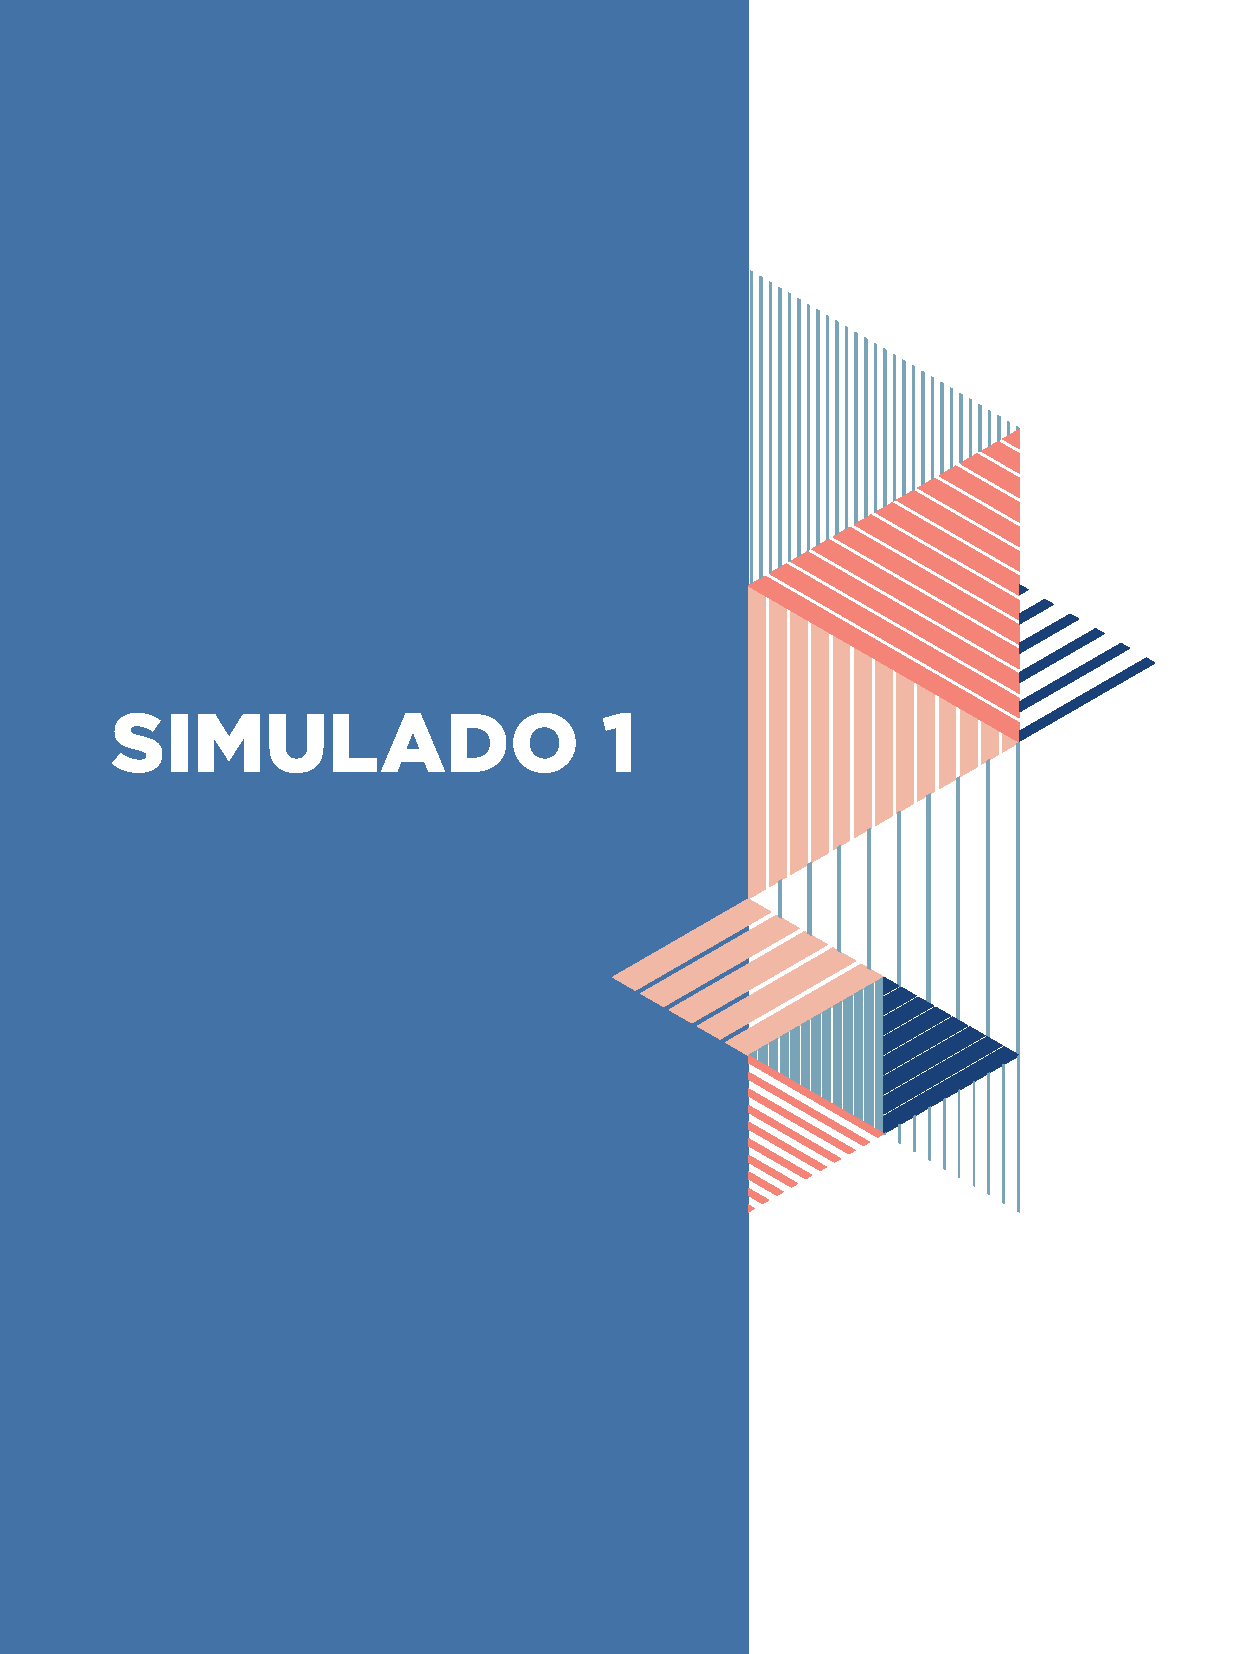
\includegraphics[scale=1]{../watermarks/1simulado9ano.pdf}
\end{figure}

\section*{Simulado 1}

\num{1}  O maior cometa já descoberto é o Holmes, que possui $2.251$ km de
diâmetro. Quantas classes possui o número que representa o diâmetro do cometa?

\begin{escolha}
\item $3$
\item $2$
\item $2.251$
\item $4$
\end{escolha}

%\subsection{BNCC: EF06MA01 }
% -- Utilizar números naturais, inteiros, racionais e
% reais, inclusive raiz quadrada, para resolver problemas com valores
% aproximados, utilizando calculadora, mentalmente ou por meio de
% estimativas, com ou sem o uso de tecnologias digitais.
% SAEB: Compor ou decompor números racionais positivos (representação
% decimal finita) na forma aditiva, ou em suas ordens, ou em adições e
% multiplicações.

% Gabarito
% Alternativa A: incorreta, pois, caso o aluno resolva transformar km em
% m, esse seria o valor, mas não é isso que o enunciado pede.
% Alternativa B: correta, pois O número $2.251$ possui $2$ classes e $4$ ordens.
% Alternativa C: incorreta, pois o aluno pode considerar que o numeral
% signifique o valor da classe, o que está incorreto.
% Alternativa D: incorreta, pois o aluno pode confundir classes com
% ordens.

\num{2}  Vilma possui um tabuleiro quadriculado com $12$ quadradinhos de largura
por $12$ quadradinhos de comprimento. Quantos quadradinhos possui o
tabuleiro de Vilma?

\begin{escolha}
\item $1$
\item $24$
\item $124$
\item $144$
\end{escolha}

%\subsection{BNCC: EF06MA06}
% : Resolver e elaborar problemas que envolvam as ideias de
% múltiplo e de divisor.
% SAEB: Calcular o resultado de adições, subtrações, multiplicações ou
% divisões envolvendo número reais.

% Gabarito
% Alternativa A: incorreta, pois o aluno pode realizar uma divisão ao
% invés da multiplicação.
% Alternativa B: incorreta, pois o aluno pode realizar uma soma ao invés
% da multiplicação.
% Alternativa C: incorreta, pois o aluno pode assinalar essa erroneamente
% por conta da semelhança em relação ao resultado correto.
% Alternativa D: correta, pois número de quadradinhos é $12$ ·12 = $144$.

\num{3}  Em um residencial serão plantadas ao lado da rua de comprimento AB.
Elas serão plantadas igualmente espaçadas como se fosse uma reta
numérica conforme a figura:

% Produzir uma figura semelhante a abaixo. Os espaços entre as árvores
% devem ser os mesmos e a quantidade de espaços não pode ser alterada.

\begin{figure}
\centering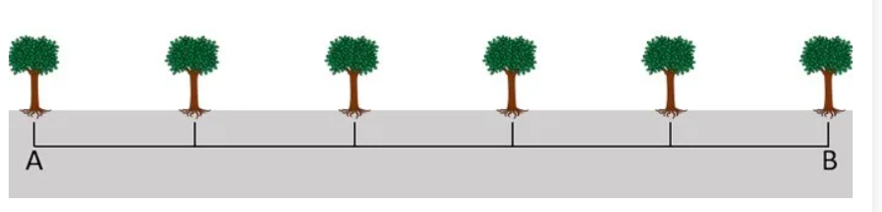
\includegraphics[width=5in,height=1.19792in]{./imgSAEB_6_MAT/media/image109.png}
\end{figure}

Qual a fração que a distância entre a primeira e a terceira árvores
representa com relação ao tamanho total?

\begin{escolha}
\item 1/4
\item 2/5
\item 1/3
\item 1/5
\end{escolha}

%\subsection{BNCC: EF06MA09}
% -- Resolver e elaborar problemas que envolvam o cálculo da
% fração de uma quantidade e cujo resultado seja um número natural, com e
% sem uso de calculadora.
% SAEB:Representar frações menores ou maiores que a unidade por meio de
% representações pictóricas ou associar frações a representações
% pictóricas.

% Gabarito
% Alternativa A: incorreta, pois o aluno pode visualizar erroneamente o
% número de arvores na figura acima e chegar a essa conclusão
% precipitadamente.
% Alternativa B: correta, pois,como o tamanho total está dividido em $5$
% partes iguais, a fração será $2/5$.
% Alternativa C: incorreta, pois o aluno pode simplesmente considerar
% todas as àrvores e chegar nesse valor.
% Alternativa D: incorreta, pois, ao contar uma árvore a menos, o aluno
% chegaria a esse valor incorretamente.

\num{4}  Um produtor vendeu sua produção no valor de $$R\$1.000,00$$ a um
feirante com $20\%$ de lucro, e este revendeu essas mercadorias com $20\,\%$
de lucro. Sendo assim o valor final da mercadoria foi de:

\begin{escolha}
\item $R\$1.020,00$
\item $R\$1.200,00$
\item $R\$1.400,00$
\item $R\$1.440,00$
\end{escolha}

%\subsection{BNCC: EF06MA13 }
% -- Resolver e elaborar problemas que envolvam
% porcentagens, com base na ideia de proporcionalidade, sem fazer uso da
% ``regra de três'', utilizando estratégias pessoais, cálculo mental e
% calculadora, em contextos de educação financeira, entre outros.
% SAEB: Resolver problemas que envolvam porcentagens, incluindo os que
% lidam com acréscimos e decréscimos simples, aplicação de percentuais
% sucessivos e determinação de taxas percentuais.

% Gabarito
% Alternativa A: incorreta, pois o aluno pode realizar uma soma ao invés
% de calcular a porcentagem e chegar a esse valor.
% Alternativa b: incorreta, pois o aluno pode realizar o cálculo de apenas
% uma parte do enunciado esquecendo o restante.
% Alternativa C: pois, o aluno pode considerar que o mesmo valor dado de
% 20\% para a primeira parte do enunciado seria o mesmo para a segunda, o
% que está equivocado.
% Alternativa D: correta, pois $1.000 x 1,2 x 1,2$ = $$R\$1.440,00$$

\num{5}  Jean foi ao supermercado e gastou $R\$19,00$ comprando seu chocolate
favorito. Se cada unidade do chocolate custa $R\$4,75$, quantos
chocolates Jean comprou?

\begin{escolha}
\item14,25
\item4
\item $23$, $75$
\item90,25
\end{escolha}

%\subsection{BNCC: EF06MA11 }
% -- Resolver e elaborar problemas com números racionais
% positivos na representação decimal, envolvendo as quatro operações
% fundamentais e a potenciação, por meio de estratégias diversas,
% utilizando estimativas e arredondamentos para verificar a razoabilidade
% de respostas, com e sem uso de calculadora.
% SAEB: Resolver problemas de adição, subtração, multiplicação, divisão,
% potenciação ou radiciação envolvendo número reais, inclusive notação
% científica.

% Gabarito
% Alternativa A: incorreta, pois o aluno pode realizar a subtração ao
% invés da divisão.
% Alternativa B: correta, pois 4,75· x = $19$; x = $4$ chocolates.
% Alternativa C: incorreta, pois o aluno pode realizar a soma ao invés da
% divisão.
% Alternativa D: incorreta, pois o aluno pode realizar a multiplicação ao
% invés da divisão.

\num{6}  Fred foi comemorar a promoção que recebeu de seu chefe em uma
pizzaria. Inicialmente resolveram pedir $3$ pizzas e perceberam que o
valor total seria de $R\$135,00$. Se após alguns cálculos resolvessem
comprar $8$ pizzas, o valor que seria pago é de:

\begin{escolha}
\item $R\$45,00$
\item $R\$135,00$
\item $R\$180,00$
\item $R\$360,00$
\end{escolha}

%\subsection{BNCC: EF06MA07 }
% -- Resolver problemas que envolvam expressões numéricas
% com números naturais e com o uso das propriedades das operações.
% SAEB: Resolver problemas de contagem cuja resolução envolva a aplicação
% do princípio multiplicativo.

% Gabarito
% Alternativa A: incorreta, pois esse seria o valor de apenas $1$ pizza.
% Alternativa B: incorreta, pois esse seria o valor de apenas $3$ pizzas.
% Alternativa C: incorreta, pois esse seria o valor de apenas $4$ pizzas.
% Alternativa D: correta, pois Valor de cada pizza: $R\$135,00/3 = R\$
% 45,00$, Valor de $8$ pizzas: $8 x 45,00 = R\$380,00$.

\num{7}  Pelas regras de um processo seletivo, o candidato que será aprovado
será aquele que tirar todas as notas acima de $30$ além disso obtiver o
maior número de notas iguais. As notas de $4$ candidatos foram colocadas
na tabela abaixo:

% %Paulo: Criar uma tabela com as informações abaixo: Candidato Português
% Matemática Direito Informática ----------- ----------- ------------
% --------- ------------- A $33$ $33$ $33$ $34$ B $32$ $39$ $32$ $40$ C $24$ $37$ $40$ $42$ D $36$
% 16 $26$ $40$

Segundo as regras do concurso, o candidato que será aprovado é a
candidato:

\begin{escolha}
\item A
\item B
\item C
\item D
\end{escolha}

%\subsection{BNCC: EF06MA19 }
% -- Resolver problemas que envolvam informações
% apresentadas em gráficos ou tabelas.
% SAEB: Inferir a finalidade da realização de uma pesquisa estatística ou
% de um levantamento, dada uma tabela (simples ou de dupla entrada) ou
% gráfico (barras simples ou agrupadas, colunas simples ou agrupadas,
% pictóricos, de linhas, de setores ou em histograma) com os dados dessa
% pesquisa.

% Gabarito
% Alternativa A: correta, pois, pela análise da tabela percebe-se que o
% candidato A teve todas as notas acima de $30$ e é o que teve mais notas
% iguais. Portanto, o candidato A deverá ser aprovado.
% Alternativa B: incorreta, pois o aluno pode observar erroneamente os
% dados da tabela e chegar a essa conclusão sem fundamentos.
% Alternativa C: incorreta, pois o aluno pode observar erroneamente os
% dados da tabela e chegar a essa conclusão sem fundamentos.
% Alternativa d: incorreta, pois o aluno pode observar erroneamente os
% dados da tabela e chegar a essa conclusão sem fundamentos.

\num{8} Uma escola fez um levantamento sobre a quantidade de alunos em dois
anos do ensino fundamental. Os dados foram apresentados no gráfico
abaixo:

\begin{figure}
\centering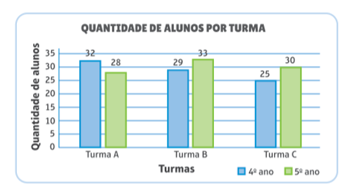
\includegraphics[width=3.78125in,height=1.94792in]{./imgSAEB_6_MAT/media/image110.png}
\end{figure}

Após analisar o gráfico, calcule e assinale a alternativa que traz o
número total de alunos do $4$º ano.

\begin{escolha}
\item $60$
\item $86$
\item $62$
\item $55$
\end{escolha}

%\subsection{BNCC: EF06MA19 }
% -- Resolver problemas que envolvam informações
% apresentadas em gráficos ou tabelas.
% SAEB: Representar ou associar os dados de uma pesquisa estatística ou de
% um levantamento em listas, tabelas (simples ou de dupla entrada) ou
% gráficos (barras simples ou agrupadas, colunas simples ou agrupadas,
% pictóricos, de linhas, de setores, ou em histograma).

% Gabarito
% Alternativa A: incorreta, pois o aluno pode considerar o valor da turma
% a como resposta.
% Alternativa B: correta, pois número de alunos do $4$º ano: $32 + 29 + 25 = 86$.
% Alternativa C: incorreta, pois o aluno pode considerar o valor da turma
% a como resposta.
% Alternativa D: incorreta, pois o aluno pode considerar o valor da turma
% a como resposta.

\num{9}  Mateus precisa ir ao dentista essa semana. Escolhendo ao acaso um dia
da semana para ir ao dentista, qual a probabilidade de Mateus escolher
uma segunda-feira ou uma quinta-feira?

\begin{escolha}
\item
  $1/7$
\item
  $2/7$
\item
  $1/5$
\item
  $2/5$
\end{escolha}


%\subsection{BNCC: EF06MA30 }
% -- Calcular a probabilidade de um evento aleatório,
% expressando-a por número racional (forma fracionária, decimal e
% percentual) e comparar esse número com a probabilidade obtida por meio
% de experimentos sucessivos.
% SAEB: Resolver problemas que envolvam a probabilidade de ocorrência de
% um resultado em eventos aleatórios equiprováveis independentes ou
% dependentes.

% Gabarito
% Alternativa A: incorreta, pois o aluno pode considerar um dia ao invés
% das duas incógnitas.
% Alternativa B: pois Dias da semana: $7$; Escolha: $2$; Probabilidade: $2/7$.
% Alternativa C: incorreta, pois o aluno pode considerar um dia do meio da
% semana encontrar erroneamente esse valor.
% Alternativa D: incorreta, pois o aluno pode considerar dois dias do meio
% da semana apenas e encontrar erroneamente esse valor.

\num{10} Uma máquina leva $6$ horas para fazer uma peça. Quantas horas ela
levará para fazer $3$ peças?

\begin{escolha}
\item $9$ horas
\item $2$ horas
\item $18$ horas
\item $216$ horas
\end{escolha}

% SAEB:Resolver problemas que envolvam variação de proporcionalidade
% direta ou inversa entre duas ou mais grandezas, inclusive escalas,
% divisões proporcionais e taxa de variação.

% Gabarito
% Alternativa A: incorreta, poic o aluno pode realizar uma soma ao invés
% de uma razão.
% Alternativa B: incorreta, pois o aluno pode realizar uma divisão ao
% invés de uma razão.
% Alternativa C: correta, pois, como cada máquina faz uma peça a cada $6$
% horas, ao triplicar a quantidade de peças iremos triplicar o tempo.
% Alternativa D: incorreta, pois o aluno pode realizar uma potenciação ao
% invés de uma razão.

\num{11} Um carro percorre $240$ km em $4$ horas. Qual é a velocidade média do
carro?

\begin{escolha}
\item $236\,km/h$
\item $60\,km/h$
\item $244\,km/h$
\item $960\,km/h$
\end{escolha}

% SAEB: Resolver problemas que envolvam variação de proporcionalidade
% direta ou inversa entre duas ou mais grandezas, inclusive escalas,
% divisões proporcionais e taxa de variação.

% Gabarito
% Alternativa A: incorreta, pois o aluno pode realizar uma subtração ao
% invés de uma razão.
% Alternativa B: correta, pois pela razão entre a distância e tempo
% teremos a velocidade.
% Alternativa C: incorreta, pois o aluno pode realizar uma soma ao invés
% de uma razão.
% Alternativa D: incorreta, pois o aluno pode realizar uma potência ao
% invés de uma razão.

\num{12} Escreva o número romano correspondente ao número decimal $1985$.

\begin{escolha}
\item MCMLXXXIII
\item MCMLXXXIV
\item MCMLXXXV
\item MCMLXXXVI
\end{escolha}

%\subsection{BNCC: EF06MA01 }
% -- Comparar, ordenar, ler e escrever números naturais e
% números racionais cuja representação decimal é finita, fazendo uso da
% reta numérica.
% SAEB: Converter uma representação de um número racional positivo para
% outra representação.

Alternativa A: incorreta, pois o aluno pode compreender erroneamente a
numeração romana e seu sistema consequentemente não tendo um fundamento
básico qualquer valor descrito nas alternativas será um valor possível
para que o aluno seja induzido a qualquer resposta.
Alternativa B: incorreta, pois o aluno pode compreender erroneamente a
numeração romana e seu sistema consequentemente não tendo um fundamento
básico qualquer valor descrito nas alternativas será um valor possível
para que o aluno seja induzido a qualquer resposta.
Alternativa C: correta, pois M = $1000$; CM = $900$; LXXX = $80$; V = $5$.
Alternativa D: incorreta, pois o aluno pode compreender erroneamente a
numeração romana e seu sistema consequentemente não tendo um fundamento
básico qualquer valor descrito nas alternativas será um valor possível
para que o aluno seja induzido a qualquer resposta.

\num{13} Uma folha de papel tem $25$ mm de largura. Qual é a medida equivalente
em centímetros?

\begin{escolha}
\item $0,0025\,cm$
\item $0,25\,cm$
\item $2,5\,cm$
\item $25\,cm$
\end{escolha}

%\subsection{BNCC: EF06MA30 }
% -- Utilizar unidades de medida padronizadas para resolver
% problemas que envolvam medidas de comprimento.
% SAEB: Resolver problemas que envolvam medidas de grandezas (comprimento,
% massa, tempo, temperatura, capacidade ou volume) em que haja conversões
% entre unidades mais usuais.

% Gabarito
% Alternativa A: incorreta, pois o aluno pode colocar erroneamente o valor
% de ``zeros'' na expressão obtendo um resultado equivocado.
% Alternativa b: incorreta, pois o aluno pode colocar erroneamente o valor
% de ``zeros'' na expressão obtendo um resultado equivocado.
% Alternativa C: correta, pois 1 cm = $10$ mm, então $25$ mm = $25 / 10 = 2,5\,cm$.
% Alternativa d: incorreta, pois o aluno pode colocar erroneamente o valor
% de ``zeros'' na expressão obtendo um resultado equivocado.

\pagebreak
\num{14} Observe a fração $1/2$. Ela pode ser representada pela figura:

\begin{figure}[h!]
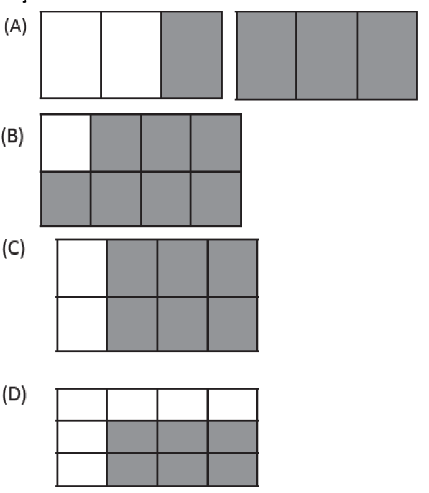
\includegraphics[width=3.57531in,height=4.10869in]{./imgSAEB_6_MAT/media/image111.png}
\end{figure}

%\subsection{BNCC: EF06MA09 }
% -- Resolver e elaborar problemas que envolvam o cálculo
% da fração de uma quantidade e cujo resultado seja um número natural, com
% e sem uso de calculadora.
% SAEB: Identificar frações equivalentes.

% Gabarito
% Alternativa A: incorreta, pois o aluno não compreendeu o conceito
% correto de $1/2$ (meio ou metade), logo, qualquer alternativa passa a ser
% válida como reposta.
% Alternativa B: incorreta, pois o aluno não compreendeu o conceito
% correto de $1/2$ (meio ou metade), logo, qualquer alternativa passa a ser
% válida como reposta.
% Alternativa C: incorreta, pois o aluno não compreendeu o conceito
% correto de $1/2$ (meio ou metade), logo, qualquer alternativa passa a ser
% válida como reposta.
% Alternativa D: correta, pois a figura representa a fração $1/2$.

\num{15} Observe a figura:

\begin{figure}[h!]
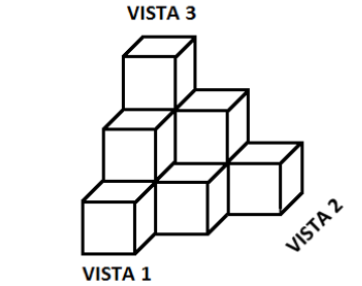
\includegraphics[width=3.01693in,height=2.38354in]{./imgSAEB_6_MAT/media/image112.png}
\end{figure}

A vista $3$ pode ser representada por:

\begin{figure}[h!]
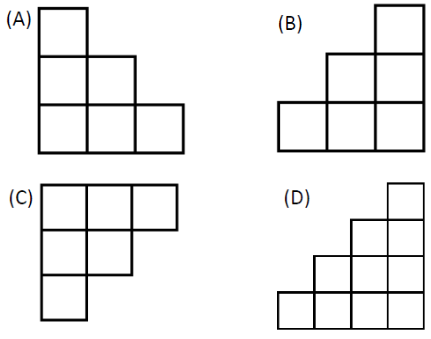
\includegraphics[width=3.59198in,height=2.82524in]{./imgSAEB_6_MAT/media/image113.png}
\end{figure}

%\subsection{BNCC: EF06MA09 }
% -- Resolver e elaborar problemas que envolvam o cálculo
% da fração de uma quantidade e cujo resultado seja um número natural, com
% e sem uso de calculadora.
% SAEB: Representar frações menores ou maiores que a unidade por meio de
% representações pictóricas ou associar frações a representações
% pictóricas.

% Gabarito
% Alternativa A: incorreta, pois a falta de adaptação a planificações e
% vistas aéreas pode levar ao aluno confusão de figuras chegando a
% assinalar essa alternativa sem compreender realmente o que a figura
% representa.
% Alternativa B: incorreta, pois a falta de adaptação a planificações e
% vistas aéreas pode levar ao aluno confusão de figuras chegando a
% assinalar essa alternativa sem compreender realmente o que a figura
% representa.
% Alternativa C: correta, pois a vista $1$ está representada na alternativa
% A, vista $2$ na alternativa B, vista $3$ na alternativa C e a alternativa D
% não representa nenhuma vista, pois tem uma sequência de $4$ blocos.
% Alternativa D: incorreta, pois a falta de adaptação a planificações e
% vistas aéreas pode levar ao aluno confusão de figuras chegando a
% assinalar essa alternativa sem compreender realmente o que a figura
% representa.

\begin{figure}[htpb!]
\vspace*{-3cm}
\hspace*{-3.7cm}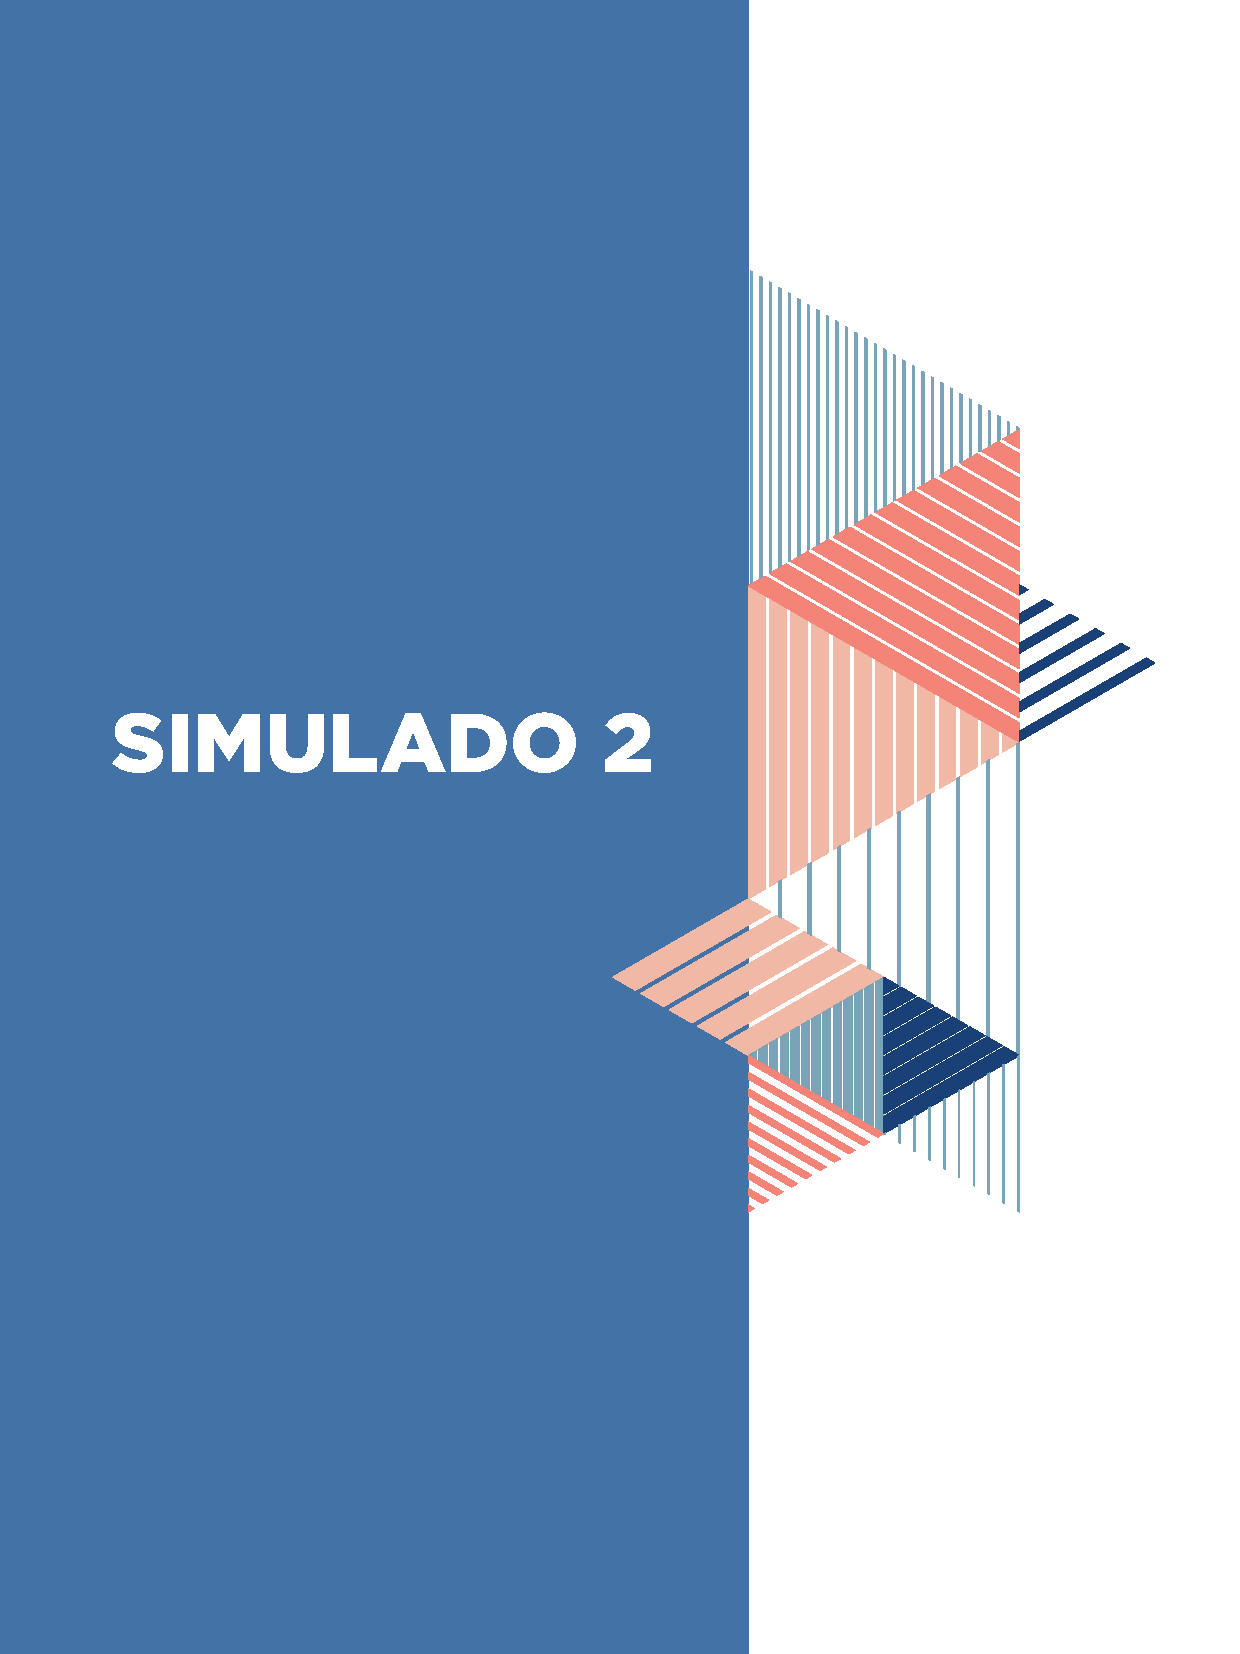
\includegraphics[scale=1]{../watermarks/2simulado9ano.pdf}
\end{figure}

\section*{Simulado 2}

\num{1}  Marcos tem três filhos cujas idades foram representadas em números
romanos:

\begin{itemize}
\item
  José tem IX anos de idade
\item
  André, o mais velho, tem XXIII anos
\item
  Joaquim, o mais novo possui VII anos de idade.
\end{itemize}

Sabendo-se que a idade de Marcos é igual a soma das idades de seus
filhos, podemos afirmar que Marcos possui:

\begin{escolha}
\item $30$ anos de idade
\item $35$ anos de idade
\item $40$ anos de idade
\item $45$ anos de idade
\end{escolha}

%\subsection{BNCC: EF06MA01 }
% -- Comparar, ordenar, ler e escrever números naturais e
% números racionais cuja representação decimal é finita, fazendo uso da
% reta numérica.
% SAEB: Escrever números racionais (representação fracionária ou decimal
% finita) em sua representação por algarismos ou em língua materna ou
% associar o registro numérico ao registro em língua materna.

% Alternativa A: incorreta, pois a conversão entre os dois sistemas
% numéricos não foi realizada corretamente
% Alternativa B: incorreta, pois a conversão entre os dois sistemas
% numéricos não foi realizada corretamente.
% Alternativa C: correta, pois X = $10$; XXIII = $23$; VII = $7$; Idade de Marcos: $10 + 23 + 7 = 40$ anos.
% Alternativa D: incorreta, pois a conversão entre os dois sistemas
% numéricos não foi realizada corretamente.

\num{2}  Entre algumas famílias foram distribuídas $240$ cadernos, $576$ lápis, e
1.080 borrachas. A distribuição foi feita de tal modo que o maior número
de famílias fosse contemplado e que cada família recebesse o mesmo
número de lápis, o mesmo número de cadernos e o mesmo número de
borrachas. Nessas condições o número de famílias que recebeu um kit
contendo lápis, borrachas e cadernos foi de:

\begin{escolha}
\item $24$
\item $28$
\item $30$
\item $42$
\end{escolha}

%\subsection{BNCC: EF06MA10 }
% -- Resolver e elaborar problemas que envolvam adição ou
% subtração com números racionais positivos na representação fracionária.
% SAEB: Resolver problemas que envolvam as ideias de múltiplo, divisor,
% máximo divisor comum ou mínimo múltiplo comum.

% Alternativa A: incorreta, pois, ao não ter um conhecimento prévio sobre
% a realização do M.\,D.\,C. como forma de resposta, qualquer alternativa
% passa a ser um resposta viável ao aluno.
% Alternativa B: incorreta, pois, ao não ter um conhecimento prévio sobre
% a realização do M.\,D.\,C. como forma de resposta, qualquer alternativa
% passa a ser um resposta viável ao aluno.
% Alternativa C: correta , pois MDC $(240; 576; 1 080) = 30$ famílias.
% Alternativa D: incorreta, pois, ao não ter um conhecimento prévio sobre
% a realização do M.\,D.\,C. como forma de resposta, qualquer alternativa
% passa a ser um resposta viável ao aluno.

\num{3} Qual é a fração geratriz da dízima periódica $0,666$\ldots?

\begin{escolha}
\item $2/3$
\item $6$/9
\item $7/10$
\item $3/4$
\end{escolha}

%SAEB: Determinar uma fração geratriz para uma dízima periódica.

% Alternativa A: correta, pois a dízima periódica em questão corresponde a
% essa fração.
% Alternativa B: incorreta, pois $6$/9: essa fração pode ser simplificada
% dividindo o numerador e o denominador por $3$, resultando em $2/3$.
% Portanto, essa é uma resposta equivocada.
% Alternativa C: incorreta, pois $7/10$: essa fração não é equivalente a
% 0,666\ldots, que é maior do que $0,7$. Portanto, essa é uma resposta
% incorreta.
% Alternativa D: incorreta, pois $3/4$: essa fração não é equivalente a
% 0,666\ldots, que é menor do que $0,75$. Portanto, essa é uma resposta
% incorreta.

\num{4}  Um círculo tem diâmetro de $8\,cm$. Qual é a medida do ângulo central
correspondente a um arco que mede $4\,cm$?

\begin{escolha}
\item $45$º
\item $60$º
\item $90$º
\item $120$º
\end{escolha}

% SAEB: Resolver problemas que envolvam relações entre os elementos de uma
% circunferência/círculo (raio, diâmetro, corda, arco, ângulo central,
% ângulo inscrito).

% Alternativa A: incorreta, pois $45$º: essa medida é obtida dividindo a
% medida do arco por metade do diâmetro, ou seja, $4$/(8/2) = $1$. Logo, o
% ângulo central correspondente seria de $1 x 180º = 180$º.
% Alternativa B: correta, pois esse é o resultado da operação.
% Alternativa C: incorreta, pois $90$º: essa medida é obtida dividindo a
% medida do arco pelo raio, ou seja, $4/4 = 1$. Logo, o ângulo central
% correspondente seria de $1 x 180º = 180$º.
% Alternativa D: incorreta, pois $120$º: essa medida é obtida dividindo a
% medida do arco por dois terços do diâmetro, ou seja, $4/((2/3) x $8$) =
% 1,5$. Logo, o ângulo central correspondente seria de $1,5 x 180º = 270$º.

\num{5}  Dois produtos químicos A e B são usados em um laboratório. Cada $1\,g$ do
produto A custa $R\$0,06$ e cada $1\,g$ do produto B custa
$R\$0,10$. Se $100\,g$ de uma mistura dos dois produtos custam $R\$7,20$, a
quantidade do produto A contida nesta mistura é:

\begin{escolha}
\item $70\,g$
\item $7,20\,g$
\item $0,60\,g$
\item $0,10\,g$
\end{escolha}

%\subsection{BNCC: EF06MA14 }
% -- Reconhecer que a relação de igualdade matemática não
% se altera ao adicionar, subtrair, multiplicar ou dividir os seus dois
% membros por um mesmo número e utilizar essa noção para determinar
% valores desconhecidos na resolução de problemas.
% SAEB: Resolver problemas que possam ser representados por sistema de
% equações de 1º grau com duas incógnitas.

% Alternativa A: correta, pois X = quantidade do produto A em gramas y = quantidade do produto B em
% gramas; A = Custo do produto A B = Custo do produto B; x + y = $100$\ldots{} (I) x·A + y·B = $7,20$\ldots{} (II); De (I), deduzimos: y = $100$ \textless{} x; Que aplicamos em (II): x·A + (100-x)·B = $7,20$; Substituindo A e B pelos seus custos em reais: x·0,06 +(100-x)·0,10 = 7,20; Multiplicando toda a equação acima por $100$, a fim de tornar inteiros seus coeficientes: $x·6 + (100-x)·10 = 720$; $6x + 1 000 - 10x = 720 -4x =$; $720 - 1000 -4x = -280 x = 70\,gramas$
% Alternativa B: incorreta, pois esse valor não corresponde aos números
% encontrados na solução da expressão.
% Alternativa C: incorreta, pois esse valor não corresponde aos números
% encontrados na solução da expressão.
% Alternativa D: incorreta, pois esse valor não corresponde aos números
% encontrados na solução da expressão.

\num{6}  Para cobrir $840\,m^2$ de um telhado, $14$ operários, que apresentam a
mesma produtividade, gastam $7$ horas. Para cobrir outros $3.360\,m^2$ do
telhado, foram contratados outros $14$ operários, que também possuem a
mesma produtividade individual dos operários anteriores. A previsão de
tempo que esses $12$ operários gastariam para realizar esse trabalho É de

\begin{escolha}
\item $3$ horas e $30$ minutos.
\item $7$ horas.
\item $14$ horas.
\item $18$ horas e $10$ minutos.
\end{escolha}

%\subsection{BNCC: EF06MA14 }
% -- Reconhecer que a relação de igualdade matemática não
% se altera ao adicionar, subtrair, multiplicar ou dividir os seus dois
% membros por um mesmo número e utilizar essa noção para determinar
% valores desconhecidos na resolução de problemas.
% SAEB: Inferir uma equação, inequação polinomial de 1º grau ou um sistema
% de equações de 1º grau com duas incógnitas que modela um problema.

% Alternativa A: incorreta, pois ,ao realizar incorretamente a montagem da
% regra de $3$, o aluno chegará a esse valor incorreto.
% Alternativa B: incorreta, pois, ao realizar incorretamente a
% multiplicação do resultado final por $2$, o aluno chegará a esse resultado
% equivocadamente.
% Alternativa C: correta.
% Alternativa D: incorreta, pois, ao realizar incorretamente a montagem da
% regra de $3$, o aluno chegará a esse valor incorreto.

% \begin{figure}
% 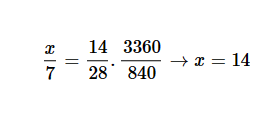
\includegraphics[width=2.76042in,height=1.20833in]{./imgSAEB_6_MAT/media/image116.png}
% \end{figure}

\num{7}  As notas de Geografia de $20$ alunos foram colocadas na tabela abaixo:

%Paulo: Criar uma tabela com as informações a seguir:

\begin{longtable}[]{@{}llllllllll@{}}
\toprule
$7,0$ & $5,0$ & $9,0$ & $5,0$ & $8,0$ & $5,0$ & $8,0$ & $9,0$ & $10,0$ &
$8,0$\tabularnewline
\midrule
\endhead
$6,0$ & $6,0$ & $7,0$ & $7,0$ & $7,0$ & $5,0$ & $5,0$ & $5,0$ & $6,0$ & $6,0$\tabularnewline
\bottomrule
\end{longtable}

Quantos alunos obtiveram nota maior ou igual a $7,0$?

\begin{escolha}
\item $8$
\item $10$
\item $9$
\item $11$
\end{escolha}

%\subsection{BNCC: EF06MA19}
% : Resolver problemas que envolvam informações apresentadas
% em gráficos ou tabelas.~
% SAEB: Argumentar ou analisar argumentações/conclusões com base nos dados
% apresentados em tabelas (simples ou de dupla entrada) ou gráficos
% (barras simples ou agrupadas, colunas simples ou agrupadas, pictóricos,
% de linhas, de setores ou em histograma).

% Alternativa A: incorreta, pois, ao visualizar $2$ valores a menos do que
% realmente está na tabela, o aluno chegará a essa conclusão erroneamente.
% Alternativa B: correta, pois entre as notas fornecidas, temos $10$ notas
% maiores ou iguais a $7,0$.
% Alternativa C: incorreta, pois, ao visualizar $1$ valor a menos do que
% realmente está na tabela, o aluno chegará a essa conclusão erroneamente.
% Alternativa D: incorreta, pois, ao visualizar $1$ valor a mais do que
% realmente está na tabela, o aluno chegará a essa conclusão erroneamente.

\num{8}  A biblioteca municipal de uma cidade do interior de São Paulo fez uma
pesquisa sobre a quantidade de livros retiradas pelas pessoas em alguns
determinados meses. Veja o resultado:

Construir um gráfico como esse, mas nos padrões do projeto.

\begin{figure}
\centering  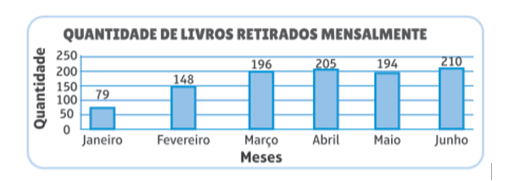
\includegraphics[width=5in,height=1.71875in]{./imgSAEB_6_MAT/media/image117.png}
\end{figure}

Pela análise dos dados a razão entre o número de livros retirados em
abril e o número de livros retirados em junho é de:

\begin{escolha}
\item $1/2$
\item $52/51$
\item $51/52$
\item $1$
\end{escolha}

%\subsection{BNCC: EF06MA19}
% SAEB: Inferir a finalidade da realização de uma pesquisa estatística ou
% de um levantamento, dada uma tabela (simples ou de dupla entrada) ou
% gráfico (barras simples ou agrupadas, colunas simples ou agrupadas,
% pictóricos, de linhas, de setores ou em histograma) com os dados dessa
% pesquisa.
%  -- Resolver problemas que envolvam informações
% apresentadas em gráficos ou tabelas.~

% Alternativa A: incorreta, pois o aluno pode considerar $2$ meses e uma
% razão e chegar nessa conclusão.
% Alternativa B: incorreta, pois o aluno pode inverter as razões e chegar
% nessa conclusão.
% Alternativa C: correta, pois $205/210 = 51/52$.
% Alternativa D: incorreta, pois o aluno pode dividir as razões e
% aproximar os valores para $1$ como resposta.

\num{9}  Qual das alternativas abaixo representa a condição de existência de
um triângulo?

\begin{escolha}
\item A soma dos ângulos internos é maior que $360$ graus. 
\item A medida de um
dos ângulos internos é igual a $90$ graus. 
\item A medida do maior lado é
igual a soma das medidas dos outros dois lados. 
\item A medida do menor
lado é igual a metade da medida da hipotenusa.
\end{escolha}

%\subsection{BNCC: EF06MA19 }
% SAEB: Identificar propriedades e relações existentes entre os elementos
% de um triângulo (condição de existência, relações de ordem entre as
% medidas dos lados e as medidas dos ângulos internos, soma dos ângulos
% internos, determinação da medida de um ângulo interno ou externo).
% -- Identificar características dos triângulos e
% classificá-los em relação às medidas dos lados e dos ângulos.

% Alternativa A: incorreta, pois a soma dos ângulos internos de um
% triângulo é igual a $180$ graus.
% Alternativa B: incorreta, pois, embora seja possível ter triângulos com
% um ângulo interno igual a $90$ graus (triângulo retângulo), essa não é uma
% condição necessária para a existência de um triângulo.
% Alternativa C: correta, pois essa é uma regra aplicada aos triângulos.
% Alternativa D: incorreta, pois essa alternativa apresenta uma informação
% contraditória, pois a hipotenusa é o maior lado em um triângulo
% retângulo, portanto não pode ser menor que um dos outros lados. Além
% disso, não há relação definida entre a medida do menor lado e a da
% hipotenusa.

\num{10} Considere um polígono com $7$ lados. É correto afirmar que:

\begin{escolha}
\item É um polígono regular.
\item É um polígono não regular.
\item É um polígono regular ou não regular, dependendo da medida dos seus
lados.
\item É um polígono regular ou não regular, dependendo da medida de seus
ângulos internos.
\end{escolha}

%\subsection{BNCC: EF06MA18}
%  -- Reconhecer, nomear e comparar polígonos, considerando
% lados, vértices e ângulos, e classificá-los em regulares e não
% regulares, tanto em suas representações no plano como em faces de
% poliedros.
% SAEB: Classificar polígonos em regulares e não regulares.

% Alternativa A: é incorreta, pois o polígono não possui lados e ângulos
% congruentes. Alternativa B: correta, pois essa é uma das características
% do polígono. Alternativa C: é incorreta, pois a medida dos lados não
% influencia na classificação do polígono como regular ou não regular.
% Alternativa D: é incorreta, pois mesmo que os ângulos internos do
% polígono sejam congruentes, ainda assim é impossível que seus lados
% sejam congruentes.

\num{11} Considere três retas paralelas cortadas por uma transversal,
formando oito ângulos. Quantos pares de ângulos são correspondentes?

\begin{escolha}
\item $2$
\item $4$
\item $6$
\item $8$
\end{escolha}

%\subsection{BNCC: EF06MA19}
% SAEB: Identificar relações entre ângulos formados por retas paralelas
% cortadas por uma transversal.
%  -- Identificar características dos triângulos e
% classificá-los em relação às medidas dos lados e dos ângulos.

% Alternativa A: incorreta, pois a alternativa afirma que existem apenas
% dois pares de ângulos correspondentes, o que está errado. Alternativa B:
% incorreta, pois a alternativa afirma que existem quatro pares de ângulos
% correspondentes, o que corresponde ao número de pares de ângulos
% correspondentes formados por duas retas paralelas cortadas por uma
% transversal, não por três retas paralelas. Alternativa C: correta, pois,
% quando uma transversal corta duas retas paralelas, cada par de ângulos
% correspondentes possui medidas iguais. Nesse caso, existem quatro pares
% de ângulos correspondentes (ângulos $1$ e $5$, $2$ e $6$, $3$ e $7$, $4$ e $8$). A
% alternativa D: incorreta, pois a alternativa afirma que existem oito
% pares de ângulos correspondentes, o que está errado.

\num{12} Qual a forma correta de escrever o número $49$ em numeração romana?

\begin{escolha}
\item XLVIX
\item LIXV
\item XLIX
\item XLIVIX
\end{escolha}

%\subsection{BNCC: EF06MA01 }
% SAEB: Comparar ou ordenar números reais, com ou sem suporte da reta
% numérica, ou aproximar número reais para múltiplos de potência de $10$
% mais próxima.
% -- Comparar, ordenar, ler e escrever números naturais e
% números racionais cuja representação decimal é finita, fazendo uso da
% reta numérica.

% Alternativa A: incorreta, o aluno pode chegar a essa conclusão
% esquecendo que que no sistema romano são apenas em casos específicos de
% impossibilidade de colocar mais de $3$ símbolos iguais para representar o
% mesmo número para inserir um número antes de outro representando uma
% subtração momentânea.
% Alternativa B: incorreta, o aluno pode chegar a essa conclusão
% esquecendo que que no sistema romano são apenas em casos específicos de
% impossibilidade de colocar mais de $3$ símbolos iguais para representar o
% mesmo número para inserir um número antes de outro representando uma
% subtração momentânea.
% Alternativa C: correta, pois 40 = XL; 9 = IX; XLIX = $40 + 9 = 49$
% Alternativa D: incorreta, pois o aluno pode chegar a essa conclusão
% esquecendo que que no sistema romano são apenas em casos específicos de
% impossibilidade de colocar mais de $3$ símbolos iguais para representar o
% mesmo número para inserir um número antes de outro representando uma
% subtração momentânea.

\num{13} Um prisma reto tem base quadrada com lado medindo $5\,cm$ e altura
medindo $8\,cm$. Qual é o seu volume?

\begin{escolha}
\item $20\,cm$³
\item $40\,cm$³
\item $100\,cm$³
\item $200\,cm$³
\end{escolha}

%\subsection{BNCC: EF06MA24 }
% SAEB: Resolver problemas que envolvam volume de prismas retos ou
% cilindros retos.
% -- Resolver e elaborar problemas que envolvam as
% grandezas comprimento, massa, tempo, temperatura, área (triângulos e
% retângulos), capacidade e volume (sólidos formados por blocos
% retangulares), sem uso de fórmulas, inseridos, sempre que possível, em
% contextos oriundos de situações reais e/ou relacionadas às outras áreas
% do conhecimento.

% Alternativa A: incorreta, pois esta alternativa corresponde ao cálculo
% do volume de um cubo cujo lado mede $2,5\,cm$, que não é o caso do prisma
% em questão.
% Alternativa B: incorreta, esta alternativa corresponde ao cálculo do
% volume de um prisma retangular com base de $5\,cm$ x $4\,cm$ e altura de $2\,cm$,
% que não é o caso do prisma em questão.
% Alternativa C: incorreta, pois esta alternativa corresponde ao cálculo
% do volume de um prisma triangular com base de $10\,cm^2$ e altura de $10\,cm$,
% que não é o caso do prisma em questão.
% Alternativa D: correta, pois a fórmula para o cálculo do volume de um
% prisma reto é dada por V = Ab x h, em que Ab é a área da base e h é a
% altura. No caso deste prisma, a base é um quadrado, cuja área é dada por
% Ab = lado². Portanto, Ab = $5^2 = 25\,cm^2$. Substituindo os valores na
% fórmula, temos: V = $25\,cm^2$ x $8\,cm$ = $200\,cm$³.

\num{14} Em uma pesquisa sobre a altura de $10$ estudantes de uma turma, os
dados obtidos foram: $1,45\,m$; $1,50\,m$; $1,60\,m$; $1,70\,m$; $1,75\,m$; $1,80\,m$;
1,85 m; $1,90\,m$; $1,95\,m$; $2,00$ m. Qual é a média aritmética simples das
alturas dos estudantes?

\begin{escolha}
\item $1,50\,m$
\item $1,75\,m$
\item $1,85\,m$
\item $1,90\,m$
\end{escolha}

%\subsection{BNCC: EF06MA32 }
% SAEB: Calcular os valores de medidas de tendência central de uma
% pesquisa estatística (média aritmética simples, moda ou mediana).
% -- Interpretar e resolver situações que envolvam dados de
% pesquisas sobre contextos ambientais, sustentabilidade, trânsito,
% consumo responsável, entre outros, apresentadas pela mídia em tabelas e
% em diferentes tipos de gráficos e redigir textos escritos com o objetivo
% de sintetizar conclusões.

% Alternativa A: incorreta, pois a média aritmética simples não é a menor
% altura nem a média entre a menor e a maior altura.
% Alternativa B: incorreta, pois a soma das alturas é maior que $17,5$ (10 x
% 1,75), portanto a média aritmética simples não pode ser menor que $1,75$.
% Alternativa C: correta, pois A média aritmética simples é obtida pela
% soma de todos os valores e divisão pelo número total de elementos.
% Portanto, somando as alturas dos $10$ estudantes, temos: $1,45 + 1,50$ +
% 1,60 + $1,70 + 1,75 + 1,80 + 1,85 + 1,90 + 1,95 + 2,00 = 18,50$ Dividindo
% esse valor por $10$, temos a média aritmética simples: $18,50 / 10 = 1,85$.
% Alternativa D: incorreta, pois A média aritmética simples é menor que a
% maior altura (2,00 m) e maior que a menor altura (1,45 m), portanto a
% alternativa d) é uma possibilidade, mas não é a resposta correta, pois a
% média aritmética simples não é a média entre a menor e a maior altura.

\num{15} Qual é a área de um retângulo de base $5\,cm$ e altura $8\,cm$?

\begin{escolha}
\item
  $13cm^2$
\item
  $35cm^2$
\item
  $40cm^2$
\item
  $56cm^2$
\end{escolha}

%\subsection{BNCC: EF06MA24 }
% SAEB: Resolver problemas que envolvam área de figuras planas.
% -- Resolver e elaborar problemas que envolvam as
% grandezas comprimento, massa, tempo, temperatura, área (triângulos e
% retângulos), capacidade e volume (sólidos formados por blocos
% retangulares), sem uso de fórmulas, inseridos, sempre que possível, em
% contextos oriundos de situações reais e/ou relacionadas às outras áreas
% do conhecimento.

% Alternativa A: incorreta, pois provavelmente houve uma confusão com os
% valores da base e da altura.
% Alternativa B: incorreta, pois o valor encontrado é menor que o produto
% dos valores da base e altura.
% Alternativa C: correta, pois a área de um retângulo é dada pelo produto
% da base pela altura, ou seja: Área = Base x Altura; Substituindo os valores dados na questão, temos: Área = $5\,cm$ x $8\,cm$ Área = $40cm^2$.
% Alternativa D: incorreta, pois o valor encontrado é maior que o produto
% dos valores da base e altura.




\pagebreak

\mbox{}

\begin{figure}
\vspace*{-3cm}
\hspace*{-3.7cm}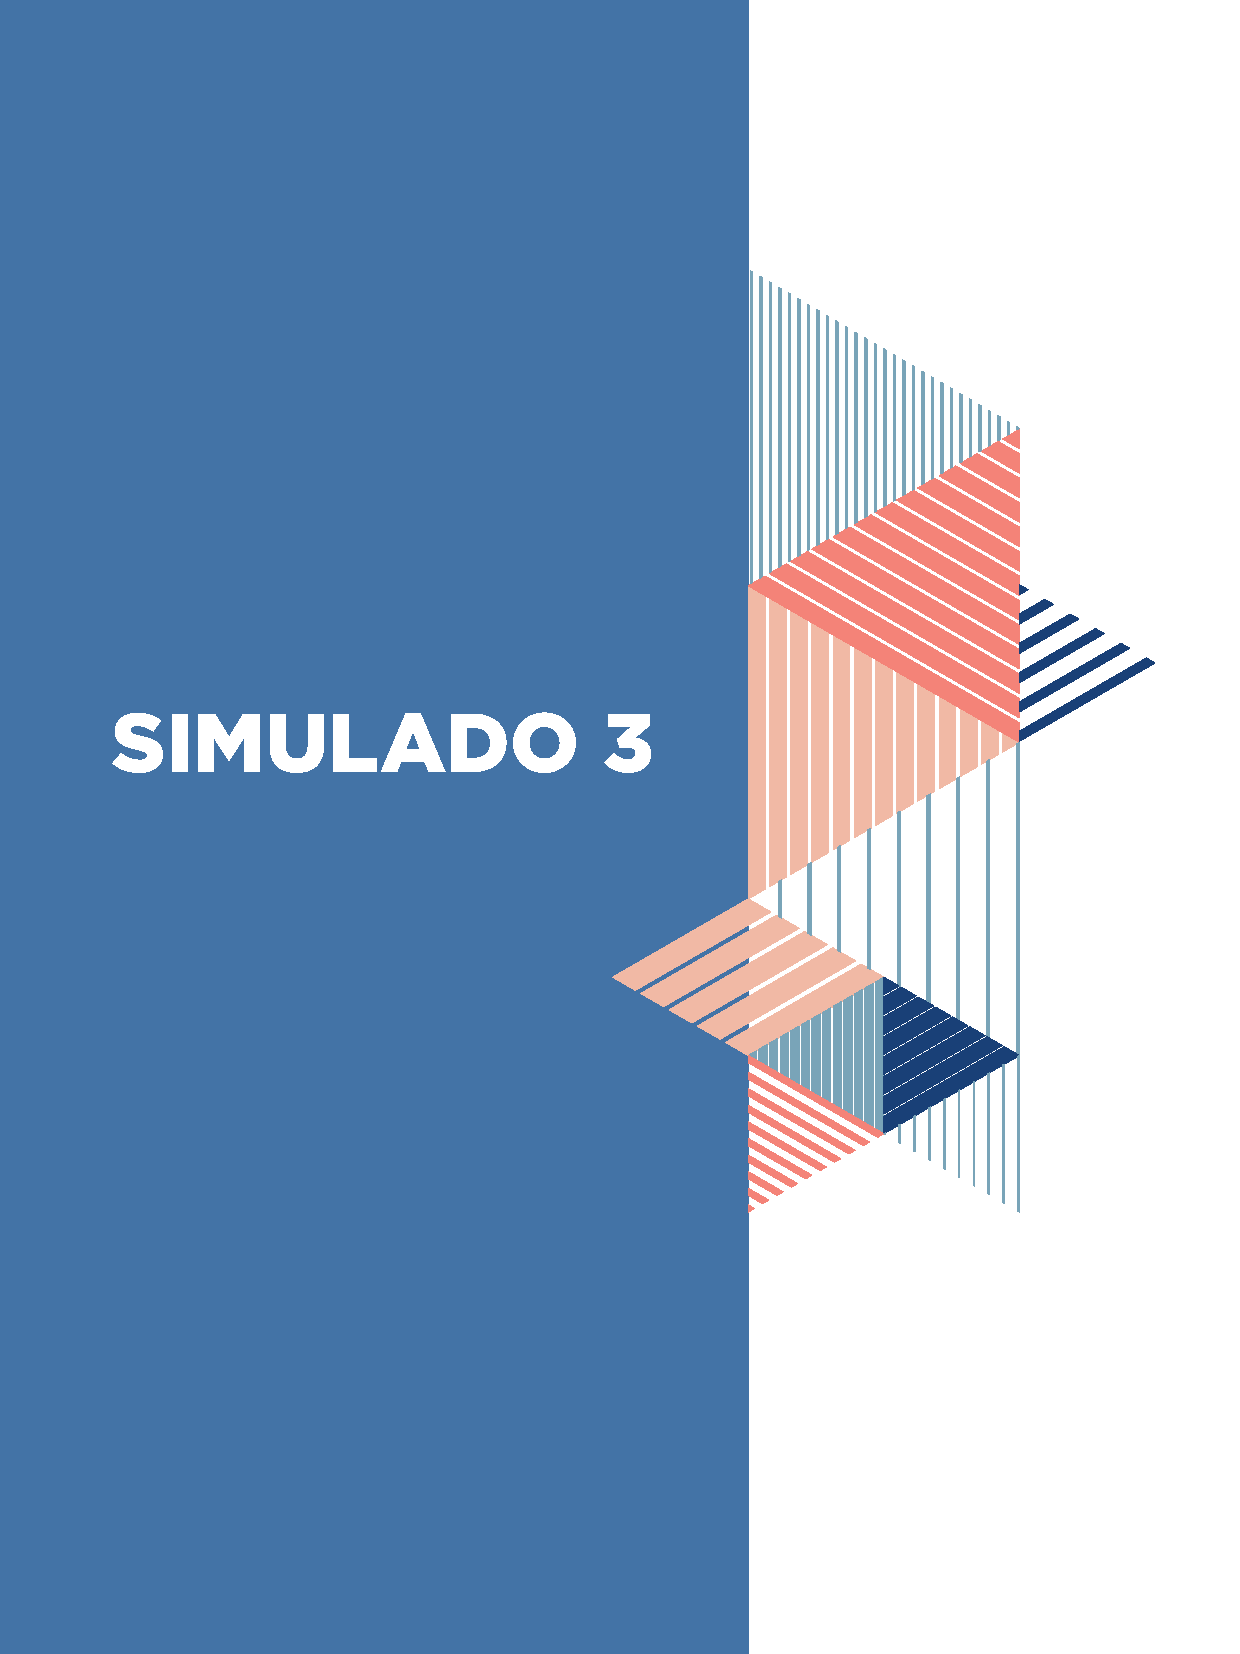
\includegraphics[scale=1]{../watermarks/3simulado9ano.pdf}
\end{figure}


\pagebreak 

\section*{Simulado 3}

\num{1}  Qual dos seguintes números é irracional?

\begin{escolha}
\item $0.5$
\item $2/3$
\item raiz quadrada de $25$
\item pi (π)
\end{escolha}

%\subsection{BNCC: EF06MA01 }
% -- Comparar, ordenar, ler e escrever números naturais e
% números racionais cuja representação decimal é finita, fazendo uso da
% reta numérica.
% SAEB: Identificar números racionais ou irracionais.

% Alternativa A: incorreta, pois $0.5$ é um número racional, podendo ser
% expresso como a fração $1/2$. Alternativa B: incorreta, pois $2/3$ é um
% número racional, já que é uma fração. Alternativa C: incorreta, pois a
% raiz quadrada de $25$ é um número inteiro. Alternativa D: correta, pois pi
% (π) é um número irracional, já que não pode ser expresso como uma fração
% finita ou decimal exata. Ele tem uma representação decimal infinita e
% não periódica, o que significa que não há um padrão repetido na
% sequência de seus dígitos.

\num{2}  Amanda abastece seu veículo a cada $5$ dias, Carlos a cada $2$ dias.
Paulo vai abastecer seu veículo sempre aos sábados e em nenhum outro
dia. Se no dia $28$ de outubro os três abasteceram seus veículos, daqui a
quantos dias eles abastecerão, novamente, no mesmo dia?

\begin{escolha}
\item $31$ dias
\item $25$ dias
\item $70$ dias
\item esse evento nunca mais acontecerá.
\end{escolha}

%\subsection{BNCC: EF06MA05 }
% SAEB: Identificar um número natural como primo, composto,
% ``múltiplo/fator de'' ou ``divisor de'' ou identificar a decomposição de
% um número natural em fatores primos ou relacionar as propriedades
% aritméticas (primo, composto, ``múltiplo/fator de'' ou ``divisor de'')
% de um número natural à sua decomposição em fatores primos.

% -- Classificar números naturais em primos e compostos,
% estabelecer relações entre números, expressas pelos termos ``é múltiplo
% de'', ``é divisor de'', ``é fator de'', e estabelecer, por meio de
% investigações, critérios de divisibilidade por $2$, $3$, $4$, $5$, $6$, $8$, $9$, $10$,
% 100 e $1000$.

% Alternativa A: incorreta, pois, por questão de semelhança, o aluno pode
% considerar que as $3$ pessoas citadas no enunciado abastecerão sempre no
% mesmo dia $28$ de todo mês.
% Alternativa B: incorreta, pois o aluno pode realizar uma soma dos dias
% ao invés de realizar o M.\,M.\,C.
% Alternativa C: correta, pois MMC(5;7,2) = $70$. 
% Alternativa D: incorreta, pois o aluno pode confundir M.\,M.\,C. por M.\,D.\,C.

\num{3} Calcule o valor da expressão: $3^2$ + raiz quadrada de $16$.

\begin{escolha}
\item $13$
\item $11$
\item $7$
\item $10$
\end{escolha}

%\subsection{BNCC: EF06MA11 }
% SAEB: Calcular o resultado de potenciação ou radiciação envolvendo
% números reais.
% -- Resolver e elaborar problemas com números racionais
% positivos na representação decimal, envolvendo as quatro operações
% fundamentais e a potenciação, por meio de estratégias diversas,
% utilizando estimativas e arredondamentos para verificar a razoabilidade
% de respostas, com e sem uso de calculadora.

% Alternativa A: incorreta, pois a resolução da expressão não corresponde
% a esse resultado.
% Alternativa B: incorreta, pois a resolução da expressão não corresponde
% a esse resultado.
% Alternativa C: incorreta, pois a resolução da expressão não corresponde
% a esse resultado.
% Alternativa D: correta pois $3^2$ significa $3$ elevado ao quadrado, ou seja,
% 3 x $3 = 9$. A raiz quadrada de $16$ é $4$. Assim, a expressão pode ser
% reescrita como $9 + 4 = 13$.

\num{4}  O número $17$ é classificado como\ldots{}

\begin{escolha}
\item
  Primo.
\item
  Composto.
\item
  Múltiplo de $3$.
\item
  Divisor de $64$.
\end{escolha}

%\subsection{BNCC: EF06MA05 }
% SAEB:Identificar um número natural como primo, composto,
% ``múltiplo/fator de'' ou ``divisor de'' ou identificar a decomposição de
% um número natural em fatores primos ou relacionar as propriedades
% aritméticas (primo, composto, ``múltiplo/fator de'' ou ``divisor de'')
% de um número natural à sua decomposição em fatores primos.
% -- Classificar números naturais em primos e compostos,
% estabelecer relações entre números, expressas pelos termos ``é múltiplo
% de'', ``é divisor de'', ``é fator de'', e estabelecer, por meio de
% investigações, critérios de divisibilidade por $2$, $3$, $4$, $5$, $6$, $8$, $9$, $10$,
% 100 e $1000$.
% EF06MA14: Resolver problemas envolvendo o cálculo de porcentagens de um
% número natural.

% Alternativa A: correta, pois m número primo é aquele que possui apenas
% dois divisores distintos: $1$ e ele mesmo. O número $17$ atende a essa
% definição, já que é divisível apenas por $1$ e por $17$.
% Alternativa B: incorreta, pois um número composto é aquele que possui
% mais de dois divisores distintos.
% Alternativa C: incorreta, pois o número $17$ não é múltiplo de $3$, já que
% não é divisível por $3$.
% Alternativa D: incorreta, pois o número $17$ não é um divisor de $64$, já
% que $64$ não é divisível por $17$.


\num{5}  Uma cerca retangular tem $10$ metros de comprimento e $6$ metros de
largura. Qual é o perímetro da cerca?

\begin{escolha}
\item $16$ m
\item $22$ m
\item $32$ m
\item $60$ m
\end{escolha}

%\subsection{BNCC: EF06MA24 }
% SAEB: Resolver problemas que envolvam perímetro de figuras planas.
% -- Resolver e elaborar problemas que envolvam as
% grandezas comprimento, massa, tempo, temperatura, área (triângulos e
% retângulos), capacidade e volume (sólidos formados por blocos
% retangulares), sem uso de fórmulas, inseridos, sempre que possível, em
% contextos oriundos de situações reais e/ou relacionadas às outras áreas
% do conhecimento.

% Alternativa A, incorreta, pois, ao aplicar a fórmula do perímetro,
% chegamos a um resultado diferente.
% Alternativa B: incorreta, pois, ao aplicar a fórmula do perímetro,
% chegamos a um resultado diferente.
% Alternativa C: correta, pois, no caso da cerca retangular descrita na
% questão, temos que ``a'' = $10$ metros e ``b'' = $6$ metros. Então, podemos
% calcular o perímetro da seguinte maneira: P = $2$a + $2$b P = $2$(10) + $2$(6) P = $20 + 12$ P = $32$.
% Alternativa D: incorreta, pois, ao aplicar a fórmula do perímetro,
% chegamos a um resultado diferente.

\num{6}  Em uma prova de matemática, $5$ alunos tiveram as seguintes notas: 5, $7$, $9$, $9$ e $10$. Qual é a média aritmética simples das notas dos alunos?

\begin{escolha}
\item $7$
\item $8$
\item $9$
\item $10$
\end{escolha}

% SAEB: Interpretar o significado das medidas de tendência central (média
% aritmética simples, moda e mediana) ou da amplitude.

% Alternativa A: incorreta, pois o cálculo da média não chega a esse
% valor.
% Alternativa B: correta, pois a média aritmética simples é a soma de
% todos os valores dividida pelo número total de valores. No caso das
% notas dos alunos, temos:
% Alternativa C: incorreta, pois o cálculo da média não chega a esse
% valor.
% Alternativa D: incorreta, pois o cálculo da média não chega a esse
% valor.

\num{7}  Quais são os passos para a realização de uma pesquisa estatística?

\begin{escolha}
\item Definição do problema, seleção da amostra, coleta de dados, análise
dos dados, conclusões e recomendações.
\item Seleção da amostra, definição do problema, coleta de dados, análise
dos dados, conclusões e recomendações.
\item Coleta de dados, definição do problema, análise dos dados, seleção da
amostra, conclusões e recomendações.
\item Análise dos dados, coleta de dados, definição do problema, seleção da
amostra, conclusões e recomendações.
\end{escolha}

%SAEB: Explicar/descrever os passos para a realização de uma pesquisa
%estatística ou de um levantamento.

% Alternativa A: correta, pois essa é a ordem correta de uma pesquisa
% estatística.
% Alternativa B: incorreta, pois o primeiro passo está na posição $2$.
% Alternativa C: incorreta, pois o primeiro passo está na posição $2$.
% Alternativa D: incorreta, pois o primeiro passo está na posição $3$.

\num{8}  Qual das alternativas abaixo associa corretamente uma equação
polinomial de 1º grau com duas variáveis a uma reta no plano cartesiano?

\begin{escolha}
\item y = $2$x - $3$ corresponde a uma reta com inclinação $2$ e intercepto no
eixo y de -3.
\item y = -3x + $2$ corresponde a uma reta com inclinação -3 e intercepto no
eixo x de $2$.
\item y = $4$x + $1$ corresponde a uma reta com inclinação $1/4$ e intercepto no
eixo y de $1$.
\item y = -x - $5$ corresponde a uma reta com inclinação -1 e intercepto no
eixo y de -5.
\end{escolha}

%\subsection{BNCC: EF06MA14}
% SAEB: Associar uma equação polinomial de 1º grau com duas variáveis a
% uma reta no plano cartesiano.
%  -- Reconhecer que a relação de igualdade matemática não
% se altera ao adicionar, subtrair, multiplicar ou dividir os seus dois
% membros por um mesmo número e utilizar essa noção para determinar
% valores desconhecidos na resolução de problemas.

% Alternativa A: correta, pois uma equação polinomial de 1º grau com duas
% variáveis, na forma y = ax + b, representa uma reta no plano cartesiano.
% O coeficiente a é a inclinação da reta e o coeficiente b é o intercepto
% no eixo y. Assim, podemos associar a equação y = $2$x - $3$ com a reta que
% passa pelo ponto (0, -3) e tem inclinação $2$. A inclinação positiva
% indica que a reta sobe da esquerda para a direita no plano cartesiano. O
% intercepto no eixo y indica que a reta cruza o eixo y no ponto (0, -3
% Alternativa B: incorreta, pois alternativa apresenta uma equação com
% inclinação negativa.
% Alternativa C: incorreta, pois a alternativa apresenta uma equação com
% inclinação diferente de $1$.
% Alternativa D: incorreta, pois a alternativa apresenta uma equação com
% inclinação diferente de $1$.

\num{9}  Qual das alternativas abaixo é a solução correta para a equação
polinomial de 1º grau $2$x + $5 = 11$?

\begin{escolha}
\item $x = 6$
\item $x = 2$
\item $x = 1,5$
\item $x = 3$
\end{escolha}

%\subsection{BNCC: EF06MA14 }
% SAEB: Resolver uma equação polinomial de 1º grau.
% -- Reconhecer que a relação de igualdade matemática não
% se altera ao adicionar, subtrair, multiplicar ou dividir os seus dois
% membros por um mesmo número e utilizar essa noção para determinar
% valores desconhecidos na resolução de problemas.

% Alternativa A: incorreta, pois a solução da expressão traz outro
% resultado.
% Alternativa B: incorreta, pois a solução da expressão traz outro
% resultado.
% Alternativa C: incorreta, pois a solução da expressão traz outro
% resultado.
% Alternativa D: correta, pois $2$x + $5 - 5 = 11 - 5$ $2$x = $6$ $2$x/2 = $6/2$ x = $3$

\num{10} Qual é a relação entre o número de vértices, faces e arestas de uma
pirâmide cuja base é um pentágono?

\begin{escolha}
\item Tem $10$ vértices, $6$ faces e $10$ arestas.
\item Tem $6$ vértices, $5$ faces e $10$ arestas.
\item Tem $6$ vértices, $6$ faces e $10$ arestas.
\item Tem $5$ vértices, $6$ faces e $10$ arestas.
\end{escolha}

%\subsection{BNCC: EF06MA17 }
% SAEB: Relacionar o número de vértices, faces ou arestas de prismas ou
% pirâmides, em função do seu polígono da base.
% -- Quantificar e estabelecer relações entre o número de
% vértices, faces e arestas de prismas e pirâmides, em função do seu
% polígono da base, para resolver problemas e desenvolver a percepção
% espacial.

% Alternativa A: incorreta, pois o número de faces está errado.
% Alternativa B: correta, pois, no caso de uma pirâmide com base
% pentagonal, o polígono da base tem $5$ lados. Cada face da pirâmide é um
% triângulo, portanto há $5$ faces triangulares. Há um vértice comum a todas
% as faces, mais $5$ vértices correspondentes aos vértices do pentágono da
% base, totalizando $6$ vértices. E como cada face tem $3$ arestas e a base
% tem $5$, há um total de $10$ arestas na pirâmide.
% Alternativa C: incorreta, pois os números de vértices e faces estão
% errados.
% Alternativa D: incorreta, pois os números de vértices e faces estão
% errados.

\num{11} Qual alternativa abaixo apresenta corretamente os elementos da
circunferência/círculo?

\begin{escolha}
\item Centro, raio, diâmetro, secante, tangente, ângulo inscrito.
\item Centro, raio, diâmetro, corda, arco, ângulo central, ângulo inscrito.
\item Centro, raio, diâmetro, corda, arco, ângulo central, ângulo externo.
\item Centro, raio, diâmetro, corda, arco, ângulo central, ângulo oposto ao
central.
\end{escolha}

%\subsection{BNCC: EF06MA18 }
% SAEB: Relacionar o número de vértices, faces ou arestas de prismas ou
% pirâmides, em função do seu polígono da base.
% -- Reconhecer, nomear e comparar polígonos, considerando
% lados, vértices e ângulos, e classificá-los em regulares e não
% regulares, tanto em suas representações no plano como em faces de
% poliedros.

% Alternativa A: incorreta, pois a alternativa menciona secante e
% tangente.
% Alternativa B: correta, pois foram mencionados todos os elementos de uma
% circunferência.
% Alternativa C: incorreta, pois a alternativa menciona ângulo externo.
% Alternativa D: incorreta, pois a alternativa menciona ângulo oposto ao
% central.

\num{12} Qual das seguintes afirmações é verdadeira sobre polígonos
semelhantes?

\begin{escolha}
\item Dois polígonos são semelhantes se têm o mesmo número de lados.
\item Dois polígonos são semelhantes se têm ângulos correspondentes
congruentes e lados correspondentes proporcionais.
\item Dois polígonos são semelhantes se têm a mesma medida de área.
\item Dois polígonos são semelhantes se têm os mesmos comprimentos de lado.
\end{escolha}

%\subsection{BNCC: EF06MA18}
% SAEB: Reconhecer polígonos semelhantes ou as relações existentes entre
% ângulos e lados correspondentes nesses tipos de polígonos.
%  -- Reconhecer, nomear e comparar polígonos, considerando
% lados, vértices e ângulos, e classificá-los em regulares e não
% regulares, tanto em suas representações no plano como em faces de
% poliedros.

% Alternativa A: incorreta, pois o número de lados não é suficiente para
% determinar se dois polígonos são semelhantes.
% Alternativa B: correta, pois dois polígonos são semelhantes se, ao
% sobrepor um sobre o outro, as medidas de seus lados correspondentes são
% multiplicadas por uma mesma constante de proporcionalidade.
% Alternativa C: incorreta, pois mesmo que dois polígonos tenham áreas
% iguais, eles não necessariamente são semelhantes.
% Alternativa D: incorreta, pois dois polígonos podem ter os mesmos
% comprimentos de lado, mas não serem semelhantes.

\num{13} Considere a figura A no plano cartesiano dada por A(2,3). Após a
aplicação da seguinte transformação geométrica, a figura A se transforma
na figura B:

Reflexão em relação ao eixo y, seguida de uma translação de $4$ unidades
para a esquerda e $2$ unidades para baixo. Qual é a coordenada da figura B no plano cartesiano?

\begin{escolha}
\item B(-6,1)
\item B(2,-5)
\item B(-2,1)
\item B(6,-1)
\end{escolha}

%\subsection{BNCC: EF06MA16 }
% SAEB: Identificar, no plano cartesiano, figuras obtidas por uma ou mais
% transformações geométricas (reflexão, translação, rotação).
% -- Associar pares ordenados de números a pontos do plano
% cartesiano do 1º quadrante, em situações como a localização dos vértices
% de um polígono.

% Alternativa A: correta, pois a reflexão em relação ao eixo y faz com que
% o ponto A(2,3) se transforme no ponto A'(-2,3). Em seguida, a translação
% de $4$ unidades para a esquerda e $2$ unidades para baixo transforma o ponto
% A'(-2,3) no ponto B(-6,1).
% Alternativa B: incorreta, pois não leva em consideração a reflexão em
% relação ao eixo y.
% Alternativa C: incorreta, pois não leva em consideração a reflexão em
% relação ao eixo y.
% Alternativa D: incorreta, pois não leva em consideração a translação de
% 4 unidades para a esquerda e $2$ unidades para baixo.

\num{14} Qual figura geométrica plana deve ser construída a partir das
seguintes condições?

Construa um triângulo equilátero com um dos lados medindo $6\,cm$.

\begin{escolha}
\item Triângulo com lados medindo $2\,cm$, $4\,cm$ e $6\,cm$. 
\item Triângulo com lados
medindo $6\,cm$, $6\,cm$ e $6\,cm$. 
\item Triângulo com lados medindo $3\,cm$, $4\,cm$ e $3\,cm$.
\item Triângulo com lados medindo $5\,cm$, $6\,cm$ e $7\,cm$.
\end{escolha}

%SAEB: Construir/desenhar figuras geométricas planas ou espaciais que
%satisfaçam condições dadas.

% Alternativa A: incorreta, pois é apresentado um triângulo com lados
% diferentes.
% Alternativa B: correta, pois Um triângulo equilátero possui os três
% lados com a mesma medida. Logo, se um dos lados mede $6\,cm$, os outros dois
% também medem $6\,cm$.
% Alternativa C: incorreta, pois é apresentado um triângulo com lados
% diferentes.
% Alternativa D: incorreta, pois é apresentado um triângulo com lados
% diferentes.

\num{15} Qual das alternativas abaixo classifica corretamente um triângulo em
relação aos seus lados?

\begin{escolha}
\item Escaleno: possui todos os lados congruentes.
\item Isósceles: possui exatamente um par de lados congruentes.
\item Equilátero: possui exatamente dois lados congruentes.
\item Retângulo: não possui um ângulo interno reto.
\end{escolha}

%\subsection{BNCC: EF06MA19 }
% SAEB: Classificar triângulos ou quadriláteros em relação aos lados ou
% aos ângulos internos.
% -- Identificar características dos triângulos e
% classificá-los em relação às medidas dos lados e dos ângulos.

% Alternativa A: incorreta, pois um triângulo escaleno não possui lados
% congruentes.
% Alternativa B: correta, pois essa é a definição de um triângulo
% isósceles.
% Alternativa C: incorreta, pois um triângulo equilátero possui todos os
% lados congruentes.
% Alternativa D: incorreta, pois triângulo retângulo possui um ângulo
% interno reto.

\pagebreak

\mbox{}

\begin{figure}
\vspace*{-3cm}
\hspace*{-3.7cm}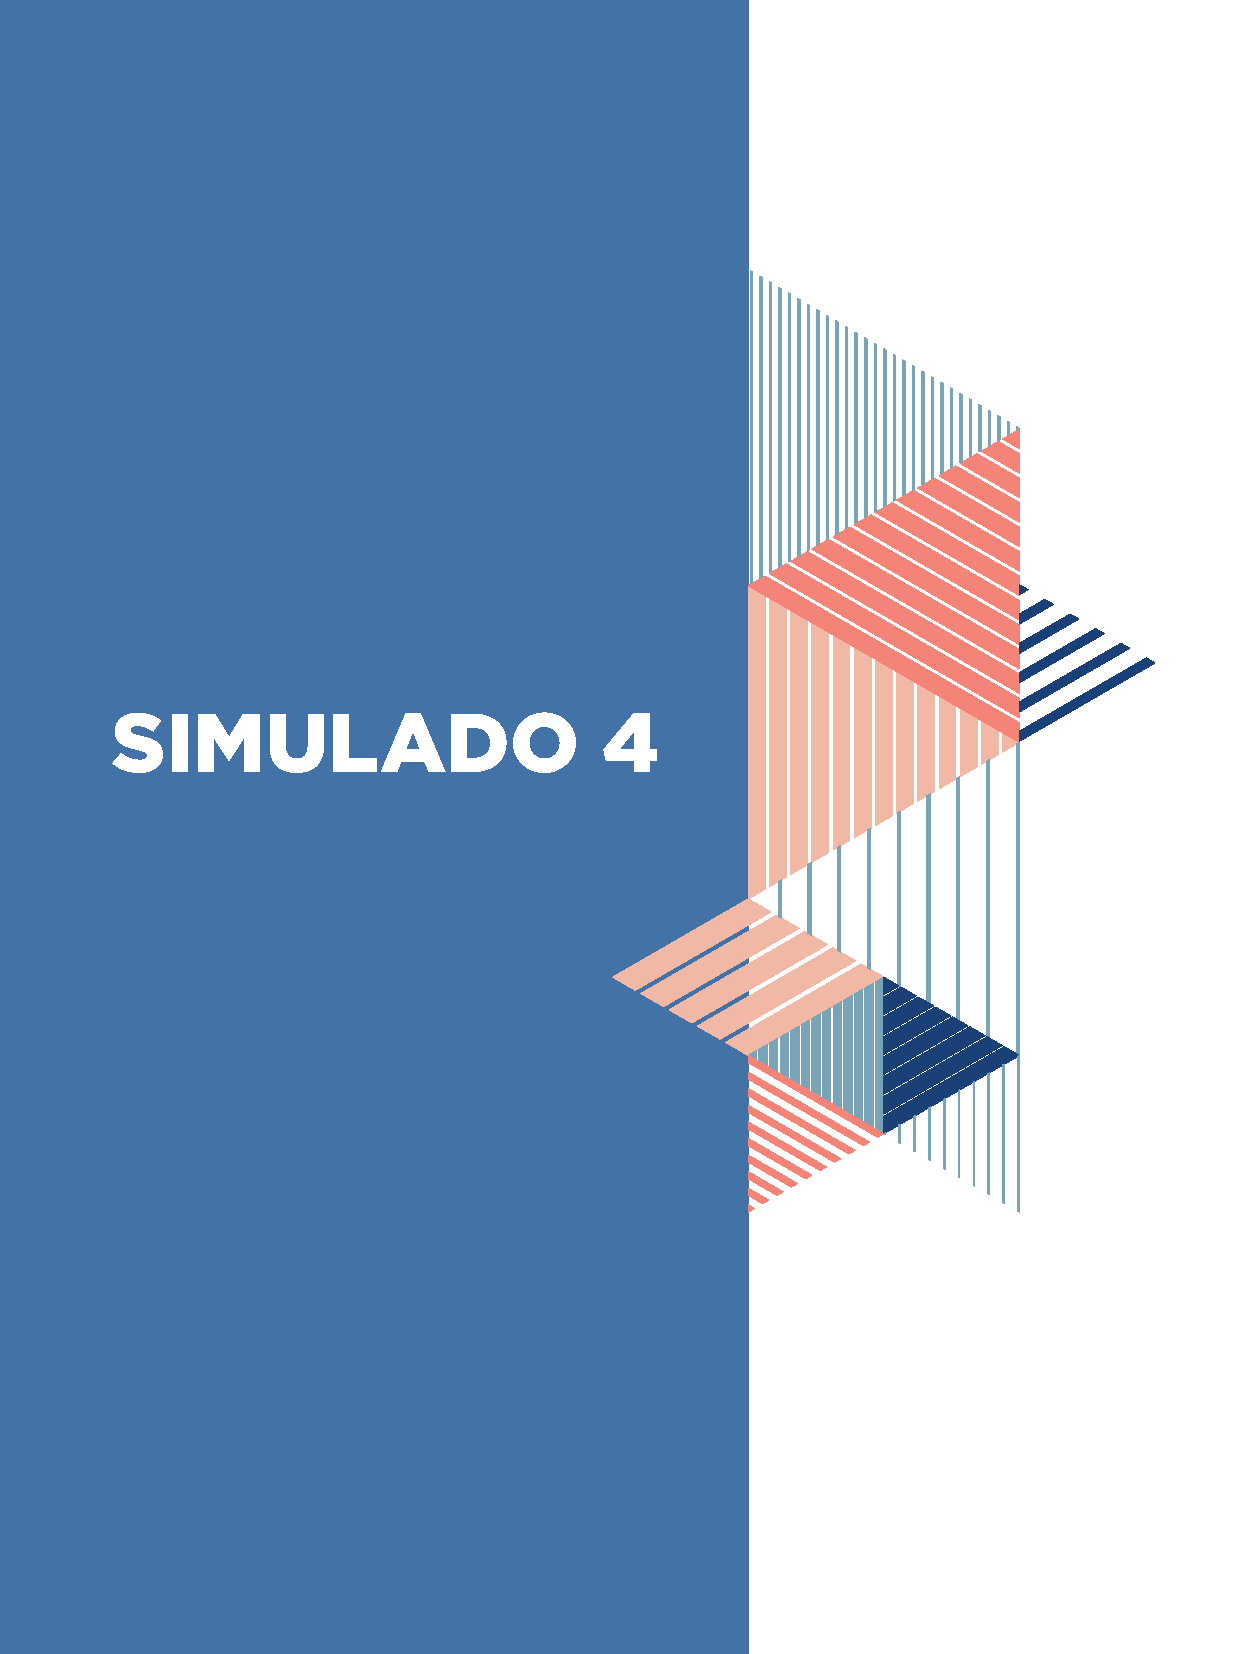
\includegraphics[scale=1]{../watermarks/4simulado9ano.pdf}
\end{figure}


\pagebreak 

\section*{Simulado 4}

\num{1}  Qual das seguintes opções corretamente identifica as relações entre
as retas e segmentos de reta no plano cartesiano?

\begin{escolha}
\item Duas retas são paralelas se possuem a mesma inclinação e intercepto y
diferente. Duas retas são perpendiculares se suas inclinações são
negativas inversas uma da outra.
\item Duas retas são concorrentes se possuem a mesma inclinação e
intercepto y diferente. Duas retas são paralelas se suas inclinações são
negativas inversas uma da outra.
\item Duas retas são perpendiculares se possuem inclinações iguais a zero e
interceptos y diferentes. Duas retas são paralelas se possuem
inclinações iguais e interceptos y diferentes.
\item Duas retas são paralelas se possuem inclinações iguais e interceptos
y diferentes. Duas retas são perpendiculares se suas inclinações são
negativas inversas uma da outra.
\end{escolha}

%\subsection{BNCC: EF06MA19 }
% SAEB: Identificar retas ou segmentos de retas concorrentes, paralelos ou
% perpendiculares.
% -- Identificar características dos triângulos e
% classificá-los em relação às medidas dos lados e dos ângulos.

% Alternativa A: incorreta, pois duas retas são paralelas se possuem a
% mesma inclinação e intercepto y iguais.
% Alternativa B: incorreta, pois duas retas são concorrentes se possuem
% inclinações diferentes, e duas retas são paralelas se possuem a mesma
% inclinação.
% Alternativa C: incorreta, pois duas retas podem ser paralelas sem ter
% inclinação igual a zero.
% Alternativa D: correta, duas retas são perpendiculares se a inclinação
% de uma é a negativa inversa da outra (isto é, seus coeficientes
% angulares multiplicados resultam em -1).

\num{2}  João precisa se deslocar do ponto A até o ponto B em um mapa, que
possui uma escala de $1\,cm$ para $5$ km. A distância entre A e B no mapa é
de $7\,cm$. Qual é a distância real que João precisa percorrer?

\begin{escolha}
\item $5$ km
\item $10$ km
\item $15$ km
\item $35$ km
\end{escolha}

%\subsection{BNCC: EF06MA21 }
% SAEB: Descrever ou esboçar deslocamento de pessoas e/ou de objetos em
% representações bidimensionais (mapas, croquis etc.), plantas de
% ambientes ou vistas, de acordo com condições dadas.
% -- Construir figuras planas semelhantes em situações de
% ampliação e de redução, com o uso de malhas quadriculadas, plano
% cartesiano ou tecnologias digitais.

% Alternativa incorreta, pois a escala indica outra relação entre as
% unidades no mapa e a distância no mundo real.
% Alternativa B: incorreta, pois a escala indica outra relação entre as
% unidades no mapa e a distância no mundo real.
% Alternativa C: incorreta, pois a escala indica outra relação entre as
% unidades no mapa e a distância no mundo real.
% Alternativa D: correta, pois a escala do mapa indica que $1\,cm$ no mapa
% representa $5$ km na realidade. 

%Portanto, se a distância entre A e B no
%mapa é de $7\,cm$, a distância real entre A e B será de:

\num{3}  Qual das seguintes opções descreve corretamente o tipo de gráfico que
deve ser utilizado para representar os dados de uma pesquisa estatística
com uma variável nominal?

\begin{escolha}
\item Gráfico de linhas
\item Gráfico de setores
\item Gráfico de barras
\item Histograma
\end{escolha}

%\subsection{BNCC: EF06MA32}
% SAEB: Representar ou associar os dados de uma pesquisa estatística ou de
% um levantamento em listas, tabelas (simples ou de dupla entrada) ou
% gráficos (barras simples ou agrupadas, colunas simples ou agrupadas,
% pictóricos, de linhas, de setores, ou em histograma).

%  -- Interpretar e resolver situações que envolvam dados de
% pesquisas sobre contextos ambientais, sustentabilidade, trânsito,
% consumo responsável, entre outros, apresentadas pela mídia em tabelas e
% em diferentes tipos de gráficos e redigir textos escritos com o objetivo
% de sintetizar conclusões.

% Alternativa A: incorreta, pois os gráficos de linhas são utilizados para
% representar dados de variáveis contínuas e quantitativas.
% Alternativa B: correta, pois o gráfico de setores (também conhecido como
% gráfico de pizza) é utilizado para representar dados de uma variável
% nominal, ou seja, dados que não têm ordem ou sequência lógica. Este tipo
% de gráfico é circular e é dividido em fatias que representam as
% diferentes categorias da variável.
% Alternativa C: incorreta, pois os gráficos de barras são usados para
% representar dados de variáveis discretas ou contínuas.
% Alternativa D: incorreta, pois o histograma é utilizado para representar
% dados de variáveis quantitativas contínuas, mas não é adequado para
% variáveis nominais.

\num{4}  Qual das alternativas abaixo melhor descreve os conceitos de
universo, variáveis e tipos de variáveis em um conjunto de dados?

\begin{escolha}
\item Universo são as amostras coletadas para uma pesquisa, variáveis são
as características das amostras coletadas e tipos de variáveis são as
formas de classificar as amostras coletadas.
\item Universo são os indivíduos ou objetos que são objetos da pesquisa,
variáveis são as características que se pretende estudar e tipos de
variáveis são a forma como essas características se manifestam.
\item Universo são as informações coletadas, variáveis são as categorias em
que essas informações são classificadas e tipos de variáveis são as
formas de visualizar essas categorias.
\item Universo são as variáveis coletadas, variáveis são as formas como
essas variáveis se relacionam e tipos de variáveis são as informações
que se pretende coletar.
\end{escolha}

%\subsection{BNCC: EF06MA31}
% SAEB: Identificar os indivíduos (universo ou população-alvo da
% pesquisa), as variáveis e os tipos de variáveis (quantitativas ou
% categóricas) em um conjunto de dados.
%  -- Identificar as variáveis e suas frequências e os
% elementos constitutivos (título, eixos, legendas, fontes e datas) em
% diferentes tipos de gráfico.

% Alternativa A: incorreta, pois o texto da alternativa apresenta
% definições erradas.
% Alternativa B: correta, pois essa alternativa apresenta a definição
% precisa dos conceitos.
% Alternativa C: incorreta, pois o texto da alternativa apresenta
% definições erradas.
% Alternativa D: incorreta, pois o texto da alternativa apresenta
% definições erradas.

\num{5}  Qual é o ponto médio do segmento de reta que tem as extremidades nos
pontos A(1, $2$) e B(5, $6$)?

\begin{escolha}
\item (2, $4$)
\item (3, $4$)
\item (4, $5$)
\item (5, $6$)
\end{escolha}

% SAEB: Determinar o ponto médio de um segmento de reta ou a distância
% entre dois pontos quaisquer, dadas as coordenadas desses pontos no plano
% cartesiano.

% Alternativa A: incorreta, pois os valores obtidos após as operações não
% correspondem à alternativa.
% Alternativa B: correta, pois o ponto médio de um segmento de reta $AB$,
% cujas coordenadas dos pontos extremos são: 
% $A(x1, y1)$ e $B(x2, y2)$, é dado pelas coordenadas do ponto $M(xm, ym)$, em que 
% $xm = (x1 + x2)/2$ e $ym = (y1 + y2)/2$. Substituindo os valores dados na questão, temos: $xm = (1 + $5$)/2 = 3$ e $ym = (2 + $6$)/2 = 4$. Portanto, o ponto médio do segmento de reta AB é $M(3, 4)$. As demais alternativas não correspondem às coordenadas do ponto médio.
% Alternativa C: incorreta, pois os valores obtidos após as operações não
% correspondem à alternativa.
% Alternativa D: incorreta, pois os valores obtidos após as operações não
% correspondem à alternativa.

\num{6}  Qual das alternativas abaixo apresenta corretamente a relação de
proporcionalidade envolvendo retas paralelas cortadas por uma
transversal?

\begin{escolha}
\item Se duas retas paralelas são cortadas por uma transversal, então as
medidas dos ângulos formados são diretamente proporcionais à distância
da transversal em relação a cada uma das retas paralelas.
\item Se duas retas paralelas são cortadas por uma transversal, então a
medida dos ângulos formados é diretamente proporcional à medida da
transversal.
\item Se duas retas paralelas são cortadas por uma transversal, então a
medida dos ângulos formados é inversamente proporcional à distância da
transversal em relação a cada uma das retas paralelas.
\item Se duas retas paralelas são cortadas por uma transversal, então a
medida dos ângulos formados é inversamente proporcional à medida da
transversal.
\end{escolha}

%SAEB: Resolver problemas que envolvam aplicação das relações de
%proporcionalidade abrangendo retas paralelas cortadas por transversais.

% Alternativa A: incorreta, pois a definição dessa relação foi descrita
% erroneamente.
% Alternativa B: incorreta, pois a definição dessa relação foi descrita
% erroneamente.
% Alternativa C: correta, pois As retas paralelas cortadas por uma
% transversal formam oito ângulos, sendo quatro pares de ângulos alternos
% internos, quatro pares de ângulos alternos externos e dois pares de
% ângulos correspondentes. Quando a transversal corta duas retas
% paralelas, a distância da transversal em relação a cada uma das retas
% paralelas é constante, portanto a relação entre as medidas dos ângulos
% formados é inversamente proporcional à distância da transversal em
% relação a cada uma das retas paralelas.
% Alternativa D: incorreta, pois a definição dessa relação foi descrita
% erroneamente.

\num{7}  Um terreno tem formato retangular e sua largura mede $20$m. Um outro
terreno, que é uma ampliação do primeiro, tem formato retangular também
e sua largura mede $30$m. Se o comprimento do primeiro terreno é de $40$m,
qual é o comprimento do segundo terreno?

\begin{escolha}
\item $60$ m
\item $80$ m
\item $120$ m
\item $150$ m
\end{escolha}

%SAEB: Resolver problemas que envolvam polígonos semelhantes.

% Alternativa A: incorreta, pois essa é a metade do comprimento do
% primeiro terreno, o que não condiz com a proporção estabelecida entre os
% terrenos.
% Alternativa B: incorreta, pois essa é uma opção que poderia ser
% confundida com a resposta correta, já que é um múltiplo do comprimento
% do primeiro terreno. No entanto, não corresponde à proporção
% estabelecida entre os terrenos.
% Alternativa C: correta, pois sabemos que os terrenos são semelhantes,
% logo, os lados correspondentes são proporcionais. Como a largura do
% segundo terreno é $1,5$ vezes maior do que a largura do primeiro (30 m/20
% m), podemos afirmar que o comprimento do segundo terreno é $1,5$ vezes
% maior do que o comprimento do primeiro terreno.
% Alternativa D: incorreta, pois essa é uma opção que poderia ser
% confundida com a resposta correta, já que é um múltiplo da largura do
% segundo terreno. No entanto, não corresponde à proporção estabelecida
% entre os terrenos.

\num{8}  Considere um triângulo ABC, onde AB = $8\,cm$, AC = $6\,cm$ e BC = $10\,cm$.
Qual é a medida da altura relativa ao lado AB?

\begin{escolha}
\item $2\,cm$
\item $3\,cm$
\item $4\,cm$
\item $5\,cm$
\end{escolha}

%\subsection{BNCC: EF06MA19}
% SAEB: Resolver problemas que envolvam relações entre ângulos formados
% por retas paralelas cortadas por uma transversal, ângulos internos ou
% externos de polígonos ou cevianas (altura, bissetriz, mediana,
% mediatriz) de polígonos.
%  -- Identificar características dos triângulos e
% classificá-los em relação às medidas dos lados e dos ângulos.

% Alternativa A: incorreta, pois $2\,cm$ é a medida da altura relativa ao
% lado BC.
% Alternativa B: incorreta, pois $3\,cm$ é a medida da altura relativa ao
% lado AC.
% Alternativa C: correta, pois a altura relativa ao lado AB divide o
% triângulo ABC em dois triângulos retângulos, onde a altura é a
% hipotenusa e os catetos são os segmentos AH e BH. Podemos utilizar o
% teorema de Pitágoras para calcular a medida da altura e chegar ao
% resultado.
% Alternativa D: incorreta, pois $5\,cm$ é a medida da mediana relativa ao
% lado AB.

\num{9}  Qual é a medida da hipotenusa de um triângulo retângulo com catetos
medindo $3\,cm$ e $4\,cm$?

\begin{escolha}
\item $5\,cm$
\item $6\,cm$
\item $7\,cm$
\item $8\,cm$
\end{escolha}

%\subsection{BNCC: EF06MA19 }
% SAEB: Resolver problemas que envolvam relações métricas do triângulo
% retângulo, incluindo o teorema de Pitágoras.
% -- Identificar características dos triângulos e
% classificá-los em relação às medidas dos lados e dos ângulos.

% Alternativa A: correta, pois pelo Teorema de Pitágoras, a soma dos
% quadrados das medidas dos catetos é igual ao quadrado da medida da
% hipotenusa. Assim, temos: $hipotenusa^2 = cateto1^2 + cateto2^2 hipotenusa^2$; $= 3^2 + 4^2 hipotenusa^2 = 9 + 16 hipotenusa^2 =$; $25 hipotenusa = 5$.
% Alternativa B: incorreta, pois esta alternativa apresenta uma medida que
% não é condizente com a aplicação do Teorema de Pitágoras.
% Alternativa C: incorreta, pois esta alternativa apresenta uma medida que
% é maior do que a hipotenusa de um triângulo retângulo formado por
% catetos medindo $3\,cm$ e $4\,cm$.
% Alternativa D: incorreta, pois esta alternativa apresenta uma medida que
% é maior do que a hipotenusa de um triângulo retângulo formado por
% catetos medindo $3\,cm$ e $4\,cm$.

\num{10} Qual é o número romano correspondente ao número $39$?

\begin{escolha}
\item XXXIX 
\item XXIX 
\item XLIX 
\item XXXVIII
\end{escolha}

%\subsection{BNCC: EF06MA01 }
% SAEB: Escrever números racionais (representação fracionária ou decimal
% finita) em sua representação por algarismos ou em língua materna ou
% associar o registro numérico ao registro em língua materna.
% -- Comparar, ordenar, ler e escrever números naturais e
% números racionais cuja representação decimal é finita, fazendo uso da
% reta numérica.

% Alternativa A: correta, pois essa é a representação correta do número.
% Alternativa B: incorreta, pois esse é o número $24$.
% Alternativa C: incorreta, pois esse é o número $49$.
% Alternativa D: incorreta, pois esse é o número $38$.

\num{11} Um campo de futebol tem $105$ m de comprimento. A medida desse campo em centímetros é igual a:

\begin{escolha}
\item $105.000\,cm$.
\item $105.000\,cm$.
\item $10.500\,cm$.
\item $1.050\,cm$.
\end{escolha}

%\subsection{BNCC: EF06MA30}
% SAEB: Resolver problemas que envolvam medidas de grandezas (comprimento,
% massa, tempo, temperatura, capacidade ou volume) em que haja conversões
% entre unidades mais usuais.
% : Utilizar unidades de medida padronizadas para resolver
% problemas que envolvam medidas de comprimento.

% Alternativa A: incorreta, pois, ao compreender erroneamente a quantidade
% de zeros a ser colocada na expressão, o aluno chegará a esse resultado.
% Alternativa B: incorreta, pois, ao compreender erroneamente a quantidade
% de zeros a ser colocada na expressão, o aluno chegará a esse resultado.
% Alternativa C: correta, pois cada metro tem $100\,cm$, desta forma $105$
% metros representam $105$·100 cm = $10.500\,cm$.
% Alternativa D: incorreta, pois, ao compreender erroneamente a quantidade
% de zeros a ser colocada na expressão, o aluno chegará a esse resultado.

\num{12} Qual é o resultado da seguinte operação: (4,5 x $10^2$) ÷ (1,5 x $10^2$)?

\begin{escolha}
\item $3$
\item $30$
\item $300$
\item $3000$
\end{escolha}

%\subsection{BNCC: EF06MA11}
% SAEB: Resolver problemas de adição, subtração, multiplicação, divisão,
% potenciação ou radiciação envolvendo número reais, inclusive notação
% científica.
%  -- Resolver e elaborar problemas com números racionais
% positivos na representação decimal, envolvendo as quatro operações
% fundamentais e a potenciação, por meio de estratégias diversas,
% utilizando estimativas e arredondamentos para verificar a razoabilidade
% de respostas, com e sem uso de calculadora.~

% Alterntiva A: incorreta, pois pois é igual ao resultado da divisão dos
% coeficientes, sem levar em conta a divisão dos expoentes.
% Alternativa B: correta, pois, para resolver a operação, é necessário
% multiplicar os números antes da divisão e depois dividir os resultados,
% obtendo: $(4,5 x 10^2) ÷ (1,5 x 10^2) = (4,5 ÷ 1,5) x (10² ÷ 10^2) = 3 x 1 = 3$.
% Alternativa C: incorreta, pois é igual à multiplicação dos coeficientes
% e dos expoentes, sem levar em conta a divisão dos coeficientes.
% Alternativa D: incorreta, pois é igual à multiplicação dos coeficientes
% e dos expoentes, sem levar em conta a divisão dos expoentes.

\num{13} Em uma fábrica de bolachas, a quantidade de bolachas produzidas é
diretamente proporcional ao número de funcionários trabalhando na linha
de produção. Se $6$ funcionários produzem $1200$ bolachas em $4$ horas,
quantas bolachas serão produzidas por $8$ funcionários em $6$ horas?

\begin{escolha}
\item $1.600$ 
\item $1.800$ 
\item $2.000$ 
\item $2.400$
\end{escolha}

% SAEB: Resolver problemas que envolvam variação de proporcionalidade
% direta ou inversa entre duas ou mais grandezas, inclusive escalas,
% divisões proporcionais e taxa de variação.

% Alternativa A: incorreta, pois não leva em conta a relação de
% proporcionalidade direta entre a quantidade de bolachas produzidas e o
% número de funcionários trabalhando na linha de produção.
% Alternativa B: incorreta, pois não leva em conta a relação de
% proporcionalidade direta entre a quantidade de bolachas produzidas e o
% número de funcionários trabalhando na linha de produção.
% Alternativa C: incorreta, pois não leva em conta a relação de
% proporcionalidade direta entre a quantidade de bolachas produzidas e o
% número de funcionários trabalhando na linha de produção.
% Alternativa D: correta, pois para $8$ funcionários em $6$ horas, temos: $8$
% funcionários x $6$ horas x $50$ bolachas por funcionário por hora = $2.400$
% bolachas.

\num{14} Em uma loja de informática, um cliente comprou $2$ teclados e $3$ mouses
por $R\$160,00$, e outro cliente comprou $3$ teclados e $2$ mouses por R\$
170,00. Qual o valor de $1$ teclado e de $1$ mouse?

\begin{escolha}
\item Teclado: $R\$50,00$ e Mouse: $R\$20,00$
\item Teclado: $R\$30,00$ e Mouse: $R\$40,00$
\item Teclado: $R\$38,00$ e Mouse: $R\$48,00$
\item Teclado: $R\$20,00$ e Mouse: $R\$50,00$
\end{escolha}

%\subsection{BNCC: EF06MA14}
% SAEB: Resolver problemas que possam ser representados por sistema de
% equações de 1º grau com duas incógnitas.
%  -- Reconhecer que a relação de igualdade matemática não
% se altera ao adicionar, subtrair, multiplicar ou dividir os seus dois
% membros por um mesmo número e utilizar essa noção para determinar
% valores desconhecidos na resolução de problemas.

% Alternativa A: incorreta, pois ao resolvermos o sistema, encontramos
% resultados diferentes.
% Alternativa B: incorreta, pois ao resolvermos o sistema, encontramos
% resultados diferentes.
% Alternativa C: correta, pois, para resolver esse problema, podemos
% utilizar um sistema de equações de 1º grau com duas incógnitas. Seja x o
% valor de um teclado e y o valor de um mouse, temos: $2x + 3y = 160$ (equação $1$) e $3x + 2y = 170$ (equação $2$). Subtraindo a equação $1$ da equação $2$, obtemos: $5x = 190$, $x = 38$. Substituindo o valor de x na equação $1$ ou na equação $2$, obtemos: $2.38 + 3y = 160$, $76 + 3y = 160$, $3y = 84, y = 28$. 
% Alternativa D: incorreta, pois ao resolvermos o sistema, encontramos
% resultados diferentes.

\num{15} Em um saco há $4$ bolas azuis, $3$ bolas vermelhas e $5$ bolas amarelas.
Se uma bola é escolhida ao acaso, qual a probabilidade de ser uma bola
azul?

\begin{escolha}
\item
  $1/4$
\item
  $1/3$
\item
  $4/12$
\item
  $6/12$
\end{escolha}

%\subsection{BNCC: EF06MA30 }


% SAEB: Resolver problemas que envolvam a probabilidade de ocorrência de
% um resultado em eventos aleatórios equiprováveis independentes ou
% dependentes.
% -- Calcular a probabilidade de um evento aleatório,
% expressando-a por número racional (forma fracionária, decimal e
% percentual) e comparar esse número com a probabilidade obtida por meio
% de experimentos sucessivos.

% Alternativa A: incorreta, pois essa fração representa a probabilidade de
% uma bola ser vermelha (3/12), não azul.
% Alternativa B: correta, pois Para calcular a probabilidade de uma bola
% ser azul, precisamos dividir o número de bolas azuis pelo número total
% de bolas no saco: Probabilidade = número de bolas azuis / número total
% de bolas Número total de bolas = $4 + 3 + 5 = 12$ Número de bolas azuis =
% 4 Probabilidade = $4/12 = 1/3$
% Alternativa C: incorreta, pois essa fração representa o número de bolas
% azuis, não a probabilidade.
% Alternativa D: incorreta, pois essa fração não é encontrada a partir do
% sistema.
